% Contributors:

% Jan Stoess <stoess@ira.uka.de>
% Simon Kellner <kellner@kit.edu>
% Konrad Miller <miller@kit.edu>
%
\documentclass[12pt, a4paper, openany]{book}
\usepackage{graphicx}
\usepackage{chngpage}
\usepackage{xspace,ifthen,epsfig}
\usepackage{cite}
\usepackage{color}
\usepackage{fancybox}
%\usepackage{pdfpages}
\usepackage{setspace}
\usepackage{subfigure}
\usepackage{longtable} 
\usepackage{tabularx} 
\usepackage{ltxtable} 
\usepackage{times}
\usepackage{url}
\usepackage{listings}
\usepackage{amsmath}
\usepackage[american,ngerman]{babel}
\usepackage[ansinew]{inputenc}
\usepackage{fancyhdr}
\usepackage{styles/kitthesiscover}
\usepackage[%dvipdfm,
   pdfauthor={Violina Zhekova},
   pdftitle={Flexible User-Friendly Trip Planning Queries},
   pdfsubject={B.sc. Thesis},
   pdfkeywords={Trip Planning}
]{hyperref}
\usepackage[ruled,linesnumbered,vlined,boxed,commentsnumbered]{algorithm2e}
\usepackage{todonotes}
\usepackage{float}
\usepackage{multirow}
\usepackage{parskip}
\usepackage{soul}
\usepackage{nameref}

\usepackage{etoolbox}
\makeatletter
\let\original@algocf@latexcaption\algocf@latexcaption
\long\def\algocf@latexcaption#1[#2]{%
	\@ifundefined{NR@gettitle}{%
		\def\@currentlabelname{#2}%
	}{%
		\NR@gettitle{#2}%
	}%
	\original@algocf@latexcaption{#1}[{#2}]%
}
\makeatother

\bibliographystyle{styles/plain}

%\raggedbottom
\newcommand{\code}[1]{{\tt \small{#1}}}
\newcommand{\evenindent}[2]{\ifodd #1 \else \hspace*{#2} \fi}

\begin{document}
\frontmatter
\unitlength1cm

\selectlanguage{american}
\setlength{\parindent}{0pt}


%% Titelseite

\title{Titel}
\author{cand. inform. Max Mustermann}
\thesistype{sa}
\primaryreviewer{Prof.\ Dr.\ Frank Bellosa}
%\secondaryreviewer{Prof.\ Dr.\ }
\advisor{Dipl.-Inform.\ Donald Duck}{}
\thesisbegindate{12.\ April 2010}
\thesisenddate{15.\ Dezember 2010}

\maketitle
\begin{otherlanguage}{ngerman}  
\thispagestyle{empty}
\vspace*{30\baselineskip}
\hbox to \textwidth{\hrulefill}
\par
\noindent Ich versichere wahrheitsgem"a"s, die Arbeit selbstst"andig verfasst, alle benutzten Hilfsmittel vollst"andig und genau angegeben und alles kenntlich gemacht zu haben, was aus Arbeiten anderer unver"andert oder mit Ab"anderungen entnommen wurde sowie die Satzung des KIT zur Sicherung guter wissenschaftlicher Praxis in der jeweils g"ultigen Fassung beachtet zu haben.\\

\noindent Karlsruhe, den \today
\end{otherlanguage}

%%%%%%%%%%%%%%%%%%%%%%%%%%%%%%%%%%%%%%%%%%%%%%%%%%%%%%%%%%%%%%%%%%%%%%%%
%% Hinweis:
%%
%% Diese Erklärung wird von der Prüfungsordnung für Diplomarbeiten 
%% verlangt und ist zu unterschreiben. Für Studienarbeiten ist diese
%% Erklärung nicht zwingend notwendig, schadet aber auch nicht.
%%%%%%%%%%%%%%%%%%%%%%%%%%%%%%%%%%%%%%%%%%%%%%%%%%%%%%%%%%%%%%%%%%%%%%%%
\clearpage







%\includepdf[page={1}]{declaration}

% Introduce the purpose, short summary of the thesis and main conclusion
\chapter{Abstract}
Trip planning queries are often from the type Sequenced Route Queries (SRQ), a form of nearest neighbor queries, which define a starting point and a list of categories to be visited in a consecutive order, given by the user. This type of queries are gaining significant interest, because of advances in location based mobile services and they are also of great importance in developing robust systems, where crisis management is of utter importance. 

Existing approaches strive to find a best route, based on length, duration or other prime factors, passing through multiple location, called Points of Interest (PoIs), and they match the route perfectly. However, users may be also interested in other qualities of the route, such as the relationship among sequence points, hierarchy, order and priority of the PoIs. Therefore, in this thesis  I introduce a set of operators, which the users may be interested in applying to SRQ, and propose approaches to designing and implementing some of the possible operators. The implementation considers metric spaces, as these are mostly relevant to the user, when working with road networks in real-life maps.
The query operators this thesis has focused on are the following: equality operator (EO), not-equality operator (NEO), or operator (OR) and order operator (ORDER). The equality operator gives the user the flexibility to build a query, where two PoIs of the same category must be equal. The not-equality answers the opposite problem. The or operator provides the user with the opportunity to give multiple variants of a SRQ, using or operands. With the order operator the user is able to assign fixed positions to one or more categories in the route query, whereas it is then no longer viewed as a sequenced route query and should thus be answered differently than a simple SRQ.

The approaches used to implement the query operators include the Progressive Neighbor Exploration (PNE) approach, presented in \cite{OSR} and heuristic methods for shrinking the search space. The extensive experiments, which were done using a real-world dataset verified that the created algorithms perform as expected and outperform the baseline approaches in terms of processing time and required workspace.

\enlargethispage{\baselineskip}

\pagebreak

\mainmatter
\addcontentsline{toc}{chapter}{Contents}
\tableofcontents

\chapter{Abbreviations}
In this chapter I introduce terms and abbreviations, often used in the context of this thesis.

Table \ref{abbr} summarizes the used abbreviations.

\begin{table}[h!]
	\centering
	\begin{tabular}{ |l|l| } 
		\hline
		\textit{Abbreviation} & \textit{Explanation} \\
		\hline
		SRQ & Sequenced Route Query \\ 

		PoI & Point of Interest \\ 

		OSR & Optimal Sequenced Route \\ 

		PNE & Progressive Neighbor Exploration \cite{OSR} \\ 

		PSR & Partial Sequenced Route \\ 

		SR & Sequenced Route (referring to full SR)\\
		
		CRQ & Complex Route Query \\
		
		EO & Equality Operator \\
		
		NEO & Not-Equality Operator \\
		
		OR & Or Operator \\
		
		ORDER & Order Operator \\
		\hline
	\end{tabular}
	\caption{Abbreviations}
	\label{abbr}
\end{table}
\chapter{Introduction}
\label{sec:intro}

\section{Motivation}
\label{sec:motivation}
A sequenced route query is defined as finding the shortest path from a starting point towards a possible destination, passing through multiple locations, defined by their category type. There has been significant research and proposed approaches on the topic, but there is not a developed query language to answer this types of queries. The work in this thesis has been focused on researching the topic of sequenced route queries and designing a language to enable the user to express his need in the form of a user query in a flexible manner, such as applying different constraints on the route to be found.

\textbf{Example:}

Figure \ref{fig:example} presents a small example network with four different types of point sets, illustrated with different colors. The colored circles represent the PoIs and the lines between them represent the roads, on each road there is a label with its length. There is two restaurants, a movie theater, two banks and two pharmacies. The starting points \textit{sp} is represented by a rhombus.

Suppose that a user is planning a trip to town: he first wants to go to a restaurant for lunch, then he wants to stop by a bank, then he meets a friend in the movie theater and after that he plans to have a dinner at a restaurant. In this specific scenario, the user wants to express his wish for the restaurant to be the same, because he may prefer a route where the equality of the two restaurant PoIs is more important to him than the length of the route.

With existing approaches, the user can get the shortest route \cite{OSR} or all routes that satisfy the semantic similarity and length conditions equally \cite{semanticSRQ}, but that does not guarantee the equality of the two restaurant PoIs. Also finding k optimal routes answering the user's SRQ and then filtering out the routes where the two PoIs of type restaurant are equal has proven to not always generate a result, which is why in this thesis a better optimal approach is presented.

Using Figure \ref{fig:example}, we see that the user query in the example above, when answered as an OSR query, delivers the route $(r_1, b_1, mt_1, r_2)$ with length 11 (shown with red lines in the figure), where both restaurants $r_1$ and $r_2$ are different. Our approach strives to find the optimal route, where the two restaurants are equal. It will not necessarily be shortest possible sequenced route, but it will be the shortest route out of all possible routes, where the two PoIs are equal to each other. Such route in our example graph would be $(r_1, b_1, mt_1, r_1)$ with length 12 (shown with dashed lines in the figure).

Specific constrains such as the equality in this example are proposed in the thesis as operators on the query. We modified and extended existing approaches, which answer the Optimal Sequenced Route (OSR) Query such as the Progressive Neighbor Exploration (PNE) \cite{OSR} in order to transform the complex user query and retrieve a desired result.

\begin{figure}[h]
	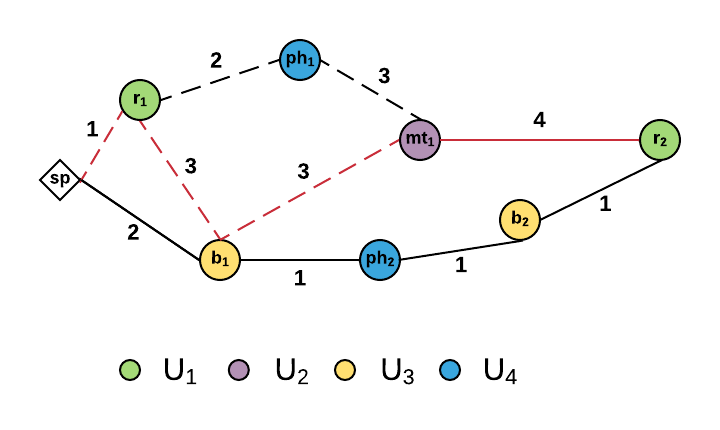
\includegraphics[scale=1]{images/Example_routes.png}
	\centering
	\caption{A network with four different types of point sets}
	\label{fig:example}
\end{figure}

\section{Problem definition}

We have a starting point and a category sequence, which constitutes the SRQ. In addition to this two query parameters, the user can define other parameters, which are applied to the route query as query operators. Such possible query operators, presented in this thesis, are the equality operator, not-equality operator, or operator and order operator. 

Then we define the \textit{Complex Route Query (CRQ)}:

\textbf{Complex route query (CRQ):} Given a starting point $sp$, a category sequence $M = (c_1, c_2, ..., c_n)$ and an operator $OPERATOR$, $Q(sp, M, OPERATOR)$ is a Complex Route (CR) Query, which searches for the optimal route $R = (r_1', r_2', ..., r_l')$, defined as a sequence of PoIs.
%Depending on which operator is applied to the query the found route $R$ follows $M$ in a way that the operator states

In Chapter \ref{sec:operators} the definitions of the separate operators are presented individually.

% e.g. performance, processing time for the trivial approach 
\section{Challenges}
When working with real-life road networks, we are usually posed with the challenge of having big datasets with many PoIs. This makes it difficult to design fast algorithms for route query problems without the need for optimizations techniques. Trivial approaches usually explore the entire dataset in order to find one optimal solution, which especially in the case of route queries can increase the time significantly. If we need to check all neighbors to one PoIs of one category and do this for all categories in order to find the shortest route from a category sequence, the time in the case of the trivial approaches increases exponentially with increase in the size of the category sequence. The \textit{Optimal Sequenced Route Query} \cite{OSR} presents the PNE approach, which solves the OSR query in metric spaces efficiently. The challenge for our task is to be able to use this designed approach to implement the proposed operators. \newline
As shown in the example in Section \ref{sec:motivation} the PNE doesn't always answer the equality operator query, therefore we modify the algorithm to serve our needs. In order to make sure that the algorithm delivers an optimal result, all routes must be checked, where two specific PoIs of one category are equal. This means that all PoIs of this category must be somehow inspected, which increases the work space significantly, which in turn spikes the processing time of the query. This poses the need for an optimization technique, such as the heuristic approach, presented in Chapter \ref{ch:EO}, to narrow the search space. \newline
The not-equality operator is an extension of the PNE algorithm, because in comparison to the equality operator, there is a greater possibility that the PNE approach finds a route with different PoIs from the same category. With a little tweak of the algorithm, it is solved by PNE without the need for an optimization technique.\newline
Furthermore, the or operator and the order operator are faced with the challenge for exponentially growing permutations, depending on the size of the query. Therefore the trivial approaches, which simply build all permutations and run PNE on them, can generate a huge work space and increase the time exponentially with the increase in the number of permutations. In our proposed approaches for these two operators we modify the PNE algorithm to be able to work on the possible permutations simultaneously, while pruning longer routes, which may be generated when the algorithm operates on the  permutations separately. In this way we shrink the search space, while also making sure, that no necessary routes are missed in the process.

% Shortly presenting the algorithms for the operators; experiment results, comparing to the baseline approach
\section{Contributions}
In this thesis, we introduce four different operators, which can be applied to a route query, and propose alternative approaches for solving them, which outperform the trivial solutions. The presented algorithms relate to the following operators: equality operator (EO), not-equality operator (NEO), or operator (OR) and order operator (ORDER). The equality operator addresses the need for flexibility, introduced in the example in Section \ref{sec:motivation}, and the not-equality solves the opposite problem, in which the user specifically wants two different PoIs of the same category type. Furthermore, the or operator represents the disjunction operator, usually present in query languages, and it gives the user the possibility to apply multiple category options to one or more route query points. Lastly, the order operator provides the user with the option to have a partially or fully not sequenced route query, where he can define zero or multiple categories to be at fixed positions in the route query sequence. \newline
The algorithms for solving the operators are largely inspired by the PNE approach, presented in the \textit{Optimal Sequenced Route Query} \cite{OSR}. For answering the equality operator query, a heuristic approach is explored, as well, for shrinking the search space and reducing the processing time. For the three of the operators (EO, OR and ORDER) baseline approaches are also introduced and compared to the proposed approaches in the experiment results. Our introduced algorithms outperform the trivial solutions in the experiments with a real dataset significantly, especially with increasing the search space with the help of different evaluation parameters, which lets us to believe that they are a meaningful way to give more flexibility to the user for different types of route queries. 

\section{Outline}
The remainder of the thesis is organized as follows: First, I review the related work that has been done on the topic of SRQ in Section 2. In Section 3 I cover the proposed operators and go into details on some of them in three separate sections for each of them: Design, Implementation and Evaluation. Finally, I conclude the thesis by summing up the progress made on the subject and discuss future work.
% This section sums up important notation, definitions, and key lemmas that are not the main focus of the thesis.
% Reformulating the OSRQuery
% Table -> summary of notations
\chapter{Notations and Preliminaries} 
\label{sec:notes}
In this chapter, I would like to introduce some terms, notations and definitions that are used throughout the thesis, such as the definition for a sequenced route query (SRQ), which we need in order to define the operators. \newline

\textbf{PoIs sets:} We assume that we have $n$ sets $U_1$, $U_2$, ..., $U_n$, which contain points in a 2-dimensional space ${\rm I\!R}^2$ and $dist(., .)$ is a distance function, which obtains the distance between two points in a two dimensional road network. The sets $U_i$ represent the data sets for the different categories of points of interest, e.g. restaurants, gas stations etc.. \newline

\textbf{Category sequence:} $M = (c_1, c_2, ..., c_l)$ is a sequence of categories, if $1 \leq M_i \leq n$ for $1 \leq i \leq l$, where n is the number of points sets $U_i$. The user is only allowed to ask for existing location types. \newline

\textbf{Route:} $R =(r_1, r_2, ..., r_r)$ is a route, if $r_i \in {\rm I\!R}^2$ for each $1 \leq i \leq r$. $R_sp$ is a route that starts from the starting point $sp$: $R_{sp} = (sp, r_1, r_2, ..., r_r)$\newline

\textbf{Route length:} The length of a route $R = (r_1, r_2, ..., r_r)$ is defined as:

\begin{equation}
length(R) = \sum_{i=1}^{r-1} dist(P_i, P_{i+1})
\end{equation}

For $r = 1$ $length(R) = 0$.
\newline

\textbf{Sequenced route:} Let $M = (c_1, c_2, ..., c_l)$ be a sequence of point of interest categories. $R = (r_1, r_2, ..., r_l)$ is a sequenced route that follows the category sequence M, if $P_i \in U_{M_i}$ where $1 \leq i \leq l$. The points of interest in the route should belong to the corresponding category sets, defined in the category sequence. \newline

\textbf{Optimal sequenced route (OSR) query:} Given a sequence of categories $M = (c_1, c_2, ..., c_l)$ and a starting point $sp$ in ${\rm I\!R}^2$, $Q(sp, M)$ is the Optimal Sequenced Route (OSR) Query, which searches for the shortest (in terms of function $length$) sequenced route $R$ that follows $M$.

\begin{equation}
length(sp, R) = dist(sp, P_1) + length(R)
\end{equation}

All other sequenced routes that follow $M$ are referred to as candidate sequenced routes (SR). \newline

Table \ref{table} summarizes all used notations.

\begin{table}[h!]
\centering
	\begin{tabular}{ |c|c| } 
		\hline
		\textit{Symbol} & \textit{Meaning} \\
		\hline
		$U_i$ & a point set for a category in ${\rm I\!R}^2$ \\ 
		\hline
		$|U_i|$ & cardinality of the set $U_i$ \\ 
		\hline
		$n$ & number of point sets $U_i$ \\ 
		\hline
		$dist(., .)$ & distance function in ${\rm I\!R}^2$ \\ 
		\hline
		$M$ & category sequence, $=(c_1, c_2, ..., c_l)$ \\ 
		\hline
		$|M|$ & $l$, size of sequence $M$ = number of items in $M$ \\ 
		\hline
		$c_i$ & $i$th member of $M$ \\ 
		\hline
		$R$ & route, $= (r_1, r_2, ..., r_r)$ \\ 
		\hline
		$|R|$ & $r$, size of route $R$ = number of points in $R$ \\ 
		\hline
		$r_i$ & $i$th point in $R$ \\ 
		\hline
		$length(R)$ & length of $R$ \\ 
		\hline
		$length(sp, R)$ & length of $R_{sp} = (sp, r_1, r_2, ..., r_r)$, $= length(R_{sp})$ \\ 
		\hline
		$Q(sp, M)$ & sequenced route query \\ 
		\hline
	\end{tabular}
\caption{Notations}
\label{table}
\end{table}





\chapter{Related Work}
\label{sec:relwork}
In this section I would like to review some existing research, related to the topic of this thesis. Sequenced route queries have been extensively researched and different algorithms that optimize the problem and address different use scenarios have been developed. Usually, existing approaches differentiate between vector and metric spaces, considering the Euclidean distance between geographic points or the real-life road-network-based distances accordingly. Some algorithms are focused on returning a single optimal route, where the PoIs match the given categories in the category sequence perfectly, whereas others consider semantic hierarchy or multiple route factors such as rating, distance and category weights. \newline

In \textit{The Optimal Sequenced Route} the researchers propose two effective algorithms for solving the sequenced route query problem. They first elaborate on why a classic shortest path algorithm such as Dijkstra would be impractical for real-life scenarios and then go on to propose the LORD (Light Optimal Route Discoverer) and R-LORD algorithm, which uses a R-tree, which are Dijkstra-based and made for vector spaces and the PNE (Progressive Neighbor Exploration) algorithm, which emplys the nearest neighbour search and is designed specifically for metric spaces. Both of their proposed algorithms calculate a perfect route and only return one optimal route (while modification of the PNE algorithm also allow for finding k optimal routes), significantly outperforming Dijkstra's algorithm. \cite{OSR}
\newline

A different approach to the SRQ, designed for metric spaces, is proposed in \textit{Sequenced Route Query with Semantic Hierarchy}. The authors suggest a Skyline based algorithm, called bulk SkySR (BSSR), which searches for all preferred routes to users by extending the shortest route search with the semantic similarity of PoIs' categories. This approach expects a category tree, representing the semantic hierarchy of categories, and applies the Skyline concept, which is searching for routes that are not worse than any other routes in terms of their scores, to the route length and semantic similarity, also known as the route scores. The BSSR algorithm also exploits the branch-and-bound concept by searching for routes simultaneously to reduce the search space. \cite{semanticSRQ}
\newline

Another research article proposes the Personalized and Sequenced Route (PSR) Query, which considers both personalization and sequenced constraints. The approach takes into account multiple factors of a route, such as distance rating and associates different weight with each PoI category and a distance weight. The framework designed to obtain one optimal route consists of three phases: guessing, crossover and refinement, and is focused on spatial databases. \cite{personalSRQ} 
\newline

In \textit{In-Route Skyline Querying for Location-Based Services} queries are issued by user moving along a routes towards destinations (PoIs), also defined as query points. The movement of the user is constrained to a road network and the travel distance is considered. In-route queries know the destination and current location of the user, which dynamically changes, and the anticipated route towards the endpoint. Users can apply weights to several spatially-related criteria, when deciding on PoIs to visit next, such as the total distance difference, known as detour, and the relative distance of the current data point. \cite{dynamicSRQ}
\newline

An article \textit{Sequenced Route Queries: Getting Things Done on the Way Back Home} suggest speedup techniques for sequenced route queries. A contraction hierarchy is proposed for preprocessing results for faster retrieval of answers by shortest path queries in road networks. The second technique uses the distance sensitivity of routes ("most queries are of a local kind"), which it bases on users' typical behavior. In this approach, one optimal route is returned, but queries where the order of PoIs is not necessarily fixed are possible as long as the number of PoIs remains moderate. Also, constraints on the order of visited PoIs can be made, e.g. visiting a restaurant before a shopping center. \cite{skyline}
\chapter{Operators} 
\label{sec:operators}

We have a starting point and a category sequence, which constitutes the SRQ. In addition to this two query parameters, the user can define other parameters, which are applied to the route query as query operators. Such possible query operators, presented in this thesis, are the equality operator, not-equality operator, or operator and order operator. 

We define the \textit{Complex Route Query} (CRQ):

\textbf{Complex route query (CRQ):} Given a starting iint $sp$, a category sequence $M = (c_1, c_2, ..., c_n)$ and an operator $OPERATOR$, $Q(sp, M, OPERATOR)$ is a Complex Route (CR) Query, which searches for the optimal route $R = (r_1', r_2', ..., r_l')$, defined as a sequence of PoIs.
%Depending on which operator is applied to the query the found route $R$ follows $M$ in a way that the operator states

In this chapter the proposed operators are covered in terms of their design, implementation and evaluation. It is divided into for subsections for each operator - EO, NEO, OR, ORDER. In the context of each operator, we first motivate the need for this operator and define it formally, then we go on to present the proposed approach and lastly we discuss the correctness of the solution and compare it with the baseline approach.

\SetKw{Return}{return}
\SetKw{Break}{break}

\SetKwFunction{PNE}{PNE}
\SetKwFunction{NN}{NN}
\SetKwFunction{KNN}{kNN}
\SetKwFunction{dist}{dist}
\SetKwFunction{length}{length}

\SetKwFunction{modifiedPNE}{modifiedPNE}
\SetKwFunction{modifiedPNE-baseline}{modifiedPNE-baseline}
\SetKwFunction{dummySR}{dummySR}
\SetKwFunction{heuristic}{heuristic}
\SetKwFunction{trim}{trim}
\SetKwFunction{caseBefore}{caseBefore}
\SetKwFunction{caseContaining}{caseContaining}
\SetKwFunction{caseAfterOrContaining}{caseAfterOrContaining}
\SetKwFunction{caseAfter}{caseAfter}

\SetKwBlock{A}{a)}{end}
\SetKwBlock{B}{b)}{end}

\section{"Equality" operator}
\label{ch:EO}

\subsection{Motivation} 
The "equality" operator is based on the need of a user to express that some PoIs of the same category in the SRQ should be equal, as presented in the example in Section \ref{sec:motivation}.

\subsection{Problem definition} 
\label{sec:problemEO}
The "equality" operator is defined as follows:

\textbf{"Equality" operator:} Given a sequence of categories $M = (c_1, c_2, ..., c_l)$, a starting point $sp$ in ${\rm I\!R}^2$ and indices $i$ and $j$, where $r_i \in C_{M_{i}}$, $r_j \in C_{M_{j}}$ and $M_i = M_j$, $EQUAL(i, j)$ is an "equality" operator, which states that $r_i$ and $r_j$ in the found route $R = (r_1, r_2, ..., r_l)$ should be the same points of interest.
$Q(sp, M, EQUAL(i, j))$ is a Sequenced Route (SR) Query, which searches for the shortest (in terms of function $length$) sequenced route $R$ that follows $M$ and where $r_i = r_j$.

\subsection{Precomputations} 
\label{sec:precompEO}
% Table with first nearest neghbors of all categories to all crossroads nodes.
In order to faster calculate the heuristic for the partial routes, the nearest neighbors of all CoIs to each node are precalculated and kept in a 2-dimensional table in memory for easy access. For precalculation a modified Dijkstra is executed for every node, which terminates as soon as it reaches the nearest neighbors of every category to a the given graph vertex.

% Introducing the proposed algorithm
\subsection{Proposed approach} 
\label{sec:approachEO}
The "equality" operator is designed using the PNE approach, proposed in \cite{OSR} and briefly presented in algorithm \texttt{\nameref{alg:PNE}}. It uses the progressive neighbor explorator as its base to upgrade on and extends it with a heuristic approach to shrink the search space.

\subsubsection{Heuristic}
\label{sec:heuristic}
For generating the routes and deciding which of them are worth further expanding on, the proposed approach uses an initially calculated \textit{upper bound} of an artificially build OSR, which satisfies the equality condition, and compares it to a lower bound of a route, considered by the algorithm. The heap is sorted by the lower bound. 

We formally define the heuristic of a route:

\textbf{\textit{Heuristic:}} Given a sequence of categories $M = (c_1, c_2, ..., c_l)$ and a PSR $R' = (r_1, r_2, ..., r_k)$ the heuristic for this route is defined as: 

\begin{equation}
h(R') = \max_{i \in [k+1, l]} nearestNeighbor(r_k, C_{M_{i}})
\end{equation}

For a full SR $h(R) = 0$.

The heuristic of a certain PSR is the maximum distance out of the distances to the nearest PoIs from the set of categories that are yet to be expanded. 

The \textbf{\textit{lower bound}} of a PSR $R'$ represents the sum of its length and its heuristic:

\begin{equation}
LB(R') = length(R') + h(R')
\end{equation}

The function \texttt{\ref{proc:heuristic}()} calculates the heuristic for a given route $R$.

\begin{function}[htb!]
\caption{heuristic($R$)}
\label{proc:heuristic}

	\tcp{Calculates the heuristic for the given route $R = (r_1, r_2, ..., r_k)$}
	\tcp{For every route, which already contains $r_i$ $R = (r_1, r_2, ...,r_i, ..., r_k)$ the distance to $r_j$ is calculated as \dist{$r_k, r_i$}}
	\For(For all direct neighbors to $r_k$ of every subsequent category find the maximum distance){$c_{k+1}$ to $c_n$}{find $h(R)$\;}	

\end{function}

% Explaining the algorithm step by step
\subsubsection{Algorithm}

The algorithm for the "equality" operator as shown in \texttt{\nameref{alg:equality}} is constructed using multiple procedures.

\begin{algorithm}[htb!]
\caption{equalityOperator()}
\label{alg:equality}
	
	\SetKwInOut{Input}{Input}
	\SetKwInOut{Output}{Output}
	
	\Input{$Q(sp, M = (c_1, c_2, ..., c_l)), EQUAL(i, j)$}
	\Output{$R = (r_1, r_2, ..., r_l)$}
	\BlankLine
	
	$initialize$ $heap$ \tcp*{Heap with PSR}
	$initialize$ $foundSR$ \tcp*{The candidate SR}
	$initialize$ $UB$\; 
	$optimalRoute \leftarrow$\PNE{$Q$}\;
	\eIf{$optimalRoute[i] = optimalRoute[j]$}{
		optimal route has been found\;
		\Return $optimalRoute$\;
	}
	{
		\dummySR{}\;
		\modifiedPNE{}\;
	}

\end{algorithm}

$heap$, $found$ and $UB$ are initialized (line 1 to 3). In $heap$ the PSR which are to be examined by the algorithm are stored. It is sorted by the \textit{lower bound} of the PSR. $foundSR$ stores a candidate SR. $UB$ is the length of the candidate route and it is updated each time a full SR is found. The update is performed in procedure \texttt{\ref{proc:trim}()}.

First, an optimal sequenced route is found using the PNE algorithm (line 4). It is checked, if the two PoIs that the user has asked to be equal (line 5), are equal in the OSR. If so, the OSR is returned (line 7), else the "equality" operator continues with the creation of an artificial SR $dummySR$ and the modified PNE algorithm (line 9, 10). 

Second, we artificially create a sequenced route from the optimal route, found by PNE, as seen in \texttt{\ref{proc:dummy}()}. The optimal route is changed, so that $r_j$ is made to be equal to $r_i$ (line 2, 3) and the length of the artificially created PSR is the initial upper bound (line 4), by which later partial sequenced routes are either kept or discarded.

\begin{procedure}[htb!]
\caption{dummySR($optimalRoute$)}
\label{proc:dummy}
	
	\tcp{Creating a dummy SR (partial sequence route) from the found optimal route; replacing $r_j$ with $r_i$}
	initiate $dummySR$ as $(r_1, r_2, ..., r_{i-1}, r_i, ..., r_i)$ \tcp*{First part of the optimal route}
	$dummySR \leftarrow add$ route found by \PNE{$r_i, (c_{j+1}, ..., c_l)$}\;
	$UB =$ \length{$dummySR$}\;
	place $dummySR$ on the $heap$\;
\end{procedure}

Then the algorithm \texttt{\nameref{alg:mPNE}} begins iterating all $r_1$ from the category set $C_{M_1}$, builds PSRs with $sp$ and each $r_1$ (line 1 to 7) and compares the \textit{lower bound}, generated by them, to the global \textit{upper bound} (line 4). The built PSRs are only considered in further steps of the algorithm, if their \textit{lower bound} is smaller than the \textit{upper bound}.

Next, the modified PNE performs as the original PNE algorithm by fetching partial sequenced routes from the $heap$ and generating new routes (line 8 to 24). This process is repeated until the $heap$ runs out of PSRs, which means that all possible candidate routes have been expanded and taken into consideration.

At each subsequent iteration of the algorithm \texttt{\nameref{alg:mPNE}} (line 9 to 26) there are four distinct cases depending on the length of the route. Case \newline \texttt{\ref{proc:c1}()} (line 11) and \texttt{\ref{proc:c4}()} (line 20) follow the original PNE. Case \texttt{\ref{proc:c2}()} (line 14) is focused on finding the travel distance between $r_{j-1}$ and $r_i$. In each of the cases after fetching the route first the \textit{lower bound} of the fetched PSR is compared to the global \textit{upper bound} to see if the route should be modified or discarded immediately (lines 1 to 3). After that the PSR is modified accordingly and again a length check is performed before finally placing the route on the $heap$. The length check is performed to make sure that the PSR is not longer than the already found SR which has a length equal to the upper bound $UB$.  

\begin{algorithm}[htb!]
\caption{modifiedPNE()}
\label{alg:mPNE}
	
	\ForEach(Checking the upper bound for every $r_1$ neighbor of $sp$ in the category set $C_{M_1}$){$r_1$ in $C_{M_1}$}{
		build a new $PSR$ with $r_1$\;
		\If{$LB(PSR) <= UB$}{
			place the new $PSR$ $(r_1)$ on the $heap$\;	
		}
	}
	
	\While{$heap$ is not empty}{
		$current \leftarrow$ fetch a $PSR$ from the $heap$\;
		\Switch{$s = size(current)$}{
			\Case(Finding PSRs before $r_j$){$s <= j-1$}{
				\caseBefore{}\;
			}
			\Case(Finding PSR containing $r_j$){$s = j$}{
				\caseContaining{}\;
			}
			\Case(Finding PSR after/containing $r_j$){$s = j+1$}{
				\caseAfterOrContaining{}\;
			}
			\Case(Finding PSRs after $r_j$){$s >= j+2$}{
				\caseAfter{}\;
			}
		}
	}
	
	\Return $foundSR$
	
\end{algorithm}

\texttt{\ref{proc:c1}()} finds PSRs before $r_j$. Two modifications of the PSR are performed, which follow the PNE algorithm. In a) (line 4 to 9) the nearest neighbor to the last PoI in the PSR $r_k$ in $C_{M_{k+1}}$ is found and the PSR is updated to contain $r_{k+1}$ and placed back on the $heap$. In b) (line 11 to 15) the k-th nearest neighbor to the second to last PoI $r_{k+1}$ in $C_{M_{k}}$ is found and the last PoIs in the PSR $r_k$ is replaced with it. \newline

\raggedbottom

\begin{procedure}[H]
\caption{caseBefore()}
\label{proc:c1}
	
	\tcp{Heuristic check}
	\If{$LB(current) <= UB$}{
		\A{
			\NN{$r_k, C_{M_{k+1}}$}\;
			update $PSR$ to contain $r_{k+1}$\;
			\tcp{Length check}
			\If{$length(PSR) <= UB$}{
				place $PSR$ on the $heap$\;
			}	
		} 
	}
	\B{
		\KNN{$r_{k-1}, C_{M_k}$}\;
		update $PSR$\;
		\If{$length(PSR) <= UB$}{
			place $PSR$ on the $heap$\;
		}	
	}
\end{procedure}

In \texttt{\ref{proc:c2}()} $r_j$ is to be found. In a) (line 4 to 10) instead of finding the nearest neighbor like the PNE algorithm does, the travel distance between the last PoI in the PSR $r_{j-1}$ and $r_i$ is calculated, because we want $r_j$ to be equal to $r_i$ in the route. In b) (line 12 to 16) the k-th nearest neighbor to the second to last PoI $r_{j-2}$ in $C_{M_{j-1}}$ is found and the last PoIs in the PSR $r_{j-1}$ is replaced with it.

\begin{procedure}[H]
\caption{caseContaining()}
\label{proc:c2}
	
	\tcp{Heuristic check}
	\If{$LB(current) <= UB$}{
		\A{
			\dist{$r_{j-1}, r_i$}\;
			update $PSR$ to contain $r_i$ in the place $j$\;
			\tcp{Length check}
			\If{$length(PSR) <= UB$}{
				\tcp{Trimming part}
				\trim{$PSR$}\;
			}
		}
	}
	\B{
		\KNN{$r_{j-2}, C_{M_{j-1}}$}\;
		update $PSR$\;
		\If{$length(PSR) <= UB$}{
			place $PSR$ on the $heap$\;
		}
	} 
\end{procedure}

\flushbottom

In \texttt{\ref{proc:c3}()} $r_{j+1}$ is to be found. In a) (line 4 to 10) the nearest neighbor to the last PoI in the PSR $r_j$ in $C_{M_{j+1}}$ is found and the PSR is updated to contain $r_{j+1}$ and placed back on the $heap$. In b) (line 12) the k-th nearest neighbor to the second to last PoI $r_{j-1}$ in $C_{M_{j-2}}$ is usually found (according ot PNE), but in our case this is $r_j$ and we have already calculated the travel distance between $r_{j-1}$ and $r_i$ in \texttt{\ref{proc:c2}()}, so here nothing further needs to be done.

\begin{procedure}[htb!]
\caption{caseAfterOrContaining()}
\label{proc:c3}
	
	\tcp{Heuristic check}
	\If{$LB(current) < UB$}{
		\A{
			\NN{$r_j, C_{M_{j+1}}$}\;
			update $PSR$ to contain $r_{j+1}$\;
			\tcp{Length check}
			\If{$length(PSR) <= UB$}{
				\tcp{Trimming part}
				\trim{$PSR$}\;
			}
		} 
	}	
	\B{
		\tcp{Already found in $caseContaning()$}
	} 
\end{procedure}

In \texttt{\ref{proc:c4}()} we find PSR after $r_j$. The case is similar to procedure \newline \texttt{\ref{proc:c1}()}, except that in a) instead of directly putting the PSR on the $heap$, trimming is performed in a) (line 10) to check if the route is a full SR and if the candidate route $foundSR$ and the upper bound $UB$ must be updated.

\begin{procedure}[htb!]
\caption{caseAfter()}
\label{proc:c4}
	
	\tcp{Same procedure as caseBefore() + trimming part to filter SR and update UB if needed}
	\tcp{Heuristic check}
	\If{$LB(current) <= UB$}{
		\A{
			\NN{$r_k, C_{M_{k+1}}$}\;
			update $PSR$ to contain $r_{k+1}$\;
			\tcp{Length check}
			\If{$length(PSR) <= UB$}{
				\tcp{Trimming part}
				\trim{$PSR$}\;
			}
		} 
	}
	\B{
		\KNN{$r_{k-1}, C_{M_k}$}\;
		update $PSR$\;
		\If{$length(PSR) <= UB$}{
			place $PSR$ on the $heap$\;
		}
	}	
\end{procedure}

\begin{algorithm}[htb!]
\caption{pne()\cite{OSR}}
\label{alg:PNE}
	
	\tcp{Incrementally create the set of candidate routes for $Q(sp, M)$ from starting point $sp$ towards CoI set $C_{M_l}$}
	\tcp{Candidate routes are stored in a heap sorted by length of the routes}
	\tcp{At each iteration of PNE a $PSR$ (partial sequenced route) is fetched and examined based on its length}
	\tcp{Trimming: There must be only one candidate SR on the $heap$}
	\Switch{$s = size(PSR)$}{
		\Case{$s == l$}{
			$PSR$ is the optimal route\;
			\Return $PSR$\;
		}
		\Case{$s \neq l$}{
			\A{
				\NN{$r_{|PSR|}, C_{M_{|PSR|+1}}$}\;
				update $PSR$ and perform trimming in case it is a candidate SR \;
				put $PSR$ back on the $heap$ \;
			} 
			\B{
				\KNN{$r_{|PSR|-1}, C_{M_{|PSR|}}$}\;
				generate a new $PSR$ and place it on the $heap$\;
			} 
		}
	}
\end{algorithm}

\begin{procedure}[H]
\caption{trim($PSR$)}
\label{proc:trim}
	
	\eIf{$size(PSR) = l$}{
		\If{$length(PSR) <= UB$}{
			update $UB$\;
			update $foundSR$\;
		}
	}{
		place $PSR$ on the $heap$\;
	}
\end{procedure}

\subsubsection{Running example}
We describe the algorithm for the "equality" operator using the example in Section \ref{sec:motivation}. The user in the example wanted to visit a restaurant, a bank, a movie theater and a restaurant again, but he wanted both restaurants to be equal ($M = (r, b, mt, r)$, $|M| = l = 4$, $EQUAL(0, 3)$). In Figure \ref{heapEO} the partial routes stored in the $heap$ in each step of the algorithm are displayed.
First, the $optimalRoute$ is found with PNE: $(r_1, b_1, mt_1, r_2)$. The algorithm checks if the PoIs at indices 0 and 3 are equal and since they are not, it continues with building the $dummySR$: $(r_1, b_1, mt_1, r_1)$. The \textit{upper bound} is initialized with the length of the $dummySR$, which is 12, and also $foundSR$ is initialized with $dummySR$ until a better route is possibly found.
In step 2 of the $modifiedPNE()$ all neighbors to the starting point $sp$ from type restaurant ($r_1$, $r_2$) are found and if their calculated $lower bound$ is smaller than the $upper bound$, which is the case for both restaurant, they are put on the $heap$: Partial routes $R_1 = (r_1)$ with length 1 and heuristic 5 and $R_2 = (r_2)$ with length 5 and heuristic 9 are generated and placed on the $heap$. Since the $heap$ is ordered ascending by $lower bound$, which is calculated as the sum of length and heuristic, $R_1$ is at the top of the $heap$ and fetched in step 3. Here we have $caseBefore()$, where we first check if the $LB$ of the PSR satisfies the condition to be smaller than the $UB$, and step a) of the PNE algorithm is performed. The nearest neighbor to $r_1$ of type bank $b_1$ is found and the new generated PSR $(r_1, b_1)$ with length 4 and heuristic 3 is calculated and placed on the $heap$. In step 4, $(r_1, b_1)$ is fetched and we enter $caseBefore()$ again and since the condition for the \textit{lower bound} to be smaller than the \textit{upper bound} is fulfilled, steps a) and b) are performed; in a) the nearest neighbor to $b_1$ from type movie theater is found, which is $mt_1$, and the PSR is extended, then in b) the next nearest neighbor to $r_1$ from type bank $b_2$ is found and a new PSR $(r_1, b_2)$ is generated. For both PSR their length is less the global \textit{upper bound} and they are put on the $heap$. The process is repeated until a route with $size(PSR) = 3$ is reached. This is the case with step 8, where we have fetches PSR $(r_1, b_1, mt_1)$. Here $caseContaining()$ is performed: the next PoI is forcefully set to be the PoI at index 0, which is $r_1$ and the travel distance from $mt_1$ to $r_1$ is calculated. $Trimming$ is performed on new SR $(r_1, b_1, mt_1, r_1)$ with length 12: it is compared with the found route and $foundSR$, but it is the same and $foundSR$ and $UB$ are not updated. In another scenario, if the newly found SR was shorter than $foundSR$, then it would be updated together with $UB$. In the next step 9, again we have $caseContaining()$ and a new full SR $(r_2, b_1, mt_1, r_2)$ with length 15 is generated, but when compared with $foundSR$, it is longer, so it gets discarded. The same steps are executed in the next two step 10 and 11, until all routes have been developed and checked, whch is the case when $heap$ is empty. Then the optimal sequenced route with equal PoIs at indices 0 and 3 in $foundSR$ is returned: $(r_1, b_1, mt_1, r_1)$.

\begin{table}[h]
	\centering
	\begin{tabular}{ |l|p{12.5cm}| } 
		\hline
		Step & Heap contents (PSR $R : length(R), heuristic(R)$) \\
		\hline
		1 & $(r_1 : 1, 5), (r_2 : 5, 4)$ \\ 
		\hline
		2 & $(r_1, b_1 : 4, 3), (r_2 : 5, 4)$ \\ 
		\hline
		3 & $(r_2 : 5, 4), (r_1, b_2 : 6, 5), (r_1, b_1, mt_1 : 7, 5)$ \\ 
		\hline
		4 & $(r_1, b_2 : 6, 5), (r_2, b_2 : 6, 5), (r_1, b_1, mt_1 : 7, 5) $ \\ 
		\hline
		5 & $(r_2, b_2 : 6, 5), (r_1, b_1, mt_1 : 7, 5) , (r_1, b_2, mt_1 : 11, 5)$ \\ 
		\hline
		6 & $(r_2, b_1 : 8, 3), (r_1, b_1, mt_1 : 7, 5) , (r_2, b_2, mt_1 : 11, 4), (r_1, b_2, mt_1 : 11, 5)$ \\ 
		\hline
		7 & $(r_1, b_1, mt_1 : 7, 5) , (r_2, b_1, mt_1 : 11, 4), (r_2, b_2, mt_1 : 11, 4), (r_1, b_2, mt_1 : 11, 5)$ \\ 
		\hline
		8 & $(r_2, b_1, mt_1 : 11, 4), (r_2, b_2, mt_1 : 11, 4), (r_1, b_2, mt_1 : 11, 5)$ \\ 
		\hline
		9 & $(r_2, b_2, mt_1 : 11, 4), (r_1, b_2, mt_1 : 11, 5)$ \\ 
		\hline
		10 & $ (r_1, b_2, mt_1 : 11, 5)$ \\ 
		\hline
		11 & $heap$ is empty \\ 
		\hline
	\end{tabular}
	\caption{Steps of the algorithm for EO using the road network from Figure \ref{fig:example}}
	\label{heapEO}
\end{table}

% Proving the correctness and comparing to the baseline/trivial approach
\subsubsection{Correctness}
We prove that our proposed approach correctly delivers a solution to the equality problem in metric spaces. In order to prove the correctness, we first prove that the heuristic is admissible.

\textbf{Lemma 1:} The heuristic, defined formally in Section \ref{sec:heuristic}, is admissible.

\textit{Proof:} For a given PSR $R' = (r_1, r_2, ..., r_k)$ let $c$ be the actual cost it takes $R'$ to be a complete route. The heuristic function $h$ would be admissible if the inequality holds:

\begin{equation}
h(R') \leq c(R')
\end{equation} 

Let us assume that $h(R') \geq c(R')$. Since we know that the heuristic is calculated as the maximum distance to the nearest neighbor of the last PoI $r_k$ to the remaining categories $(c_{k+1}, ..., c_l)$ in $M$, we are certain that the route will have at least actual cost $c(R')$ the heuristic $h(R')$ itself. It is not possible that the actual cost would exceed the heuristic, because then the $h(R')$ could not be a distance to a nearest neighbor. Therefore the equation holds true by contradiction and we proved the heuristic to be admissible. With this we know that the \textit{lower bound} of $R'$, which is calculated as $length(R') + h(R')$ could not be overestimated and thus an estimated optimal path is found.

Next we need to prove that no suitable partial sequenced routes are pruned by the proposed algorithm.

\textbf{Lemma 2:} For given query $Q(sp, M, EQUAL(i, j))$, the algorithm for the "equality" operator returns an optimal route in terms of route length.

\textit{Proof by contradiction:} Let $R' = (r_1', r_2', ..., r_l')$ to be the optimal route and $R = (r_1, r_2, ..., r_l)$ to be the route that the algorithm finds. We assume $length(R') < length(R)$ and show that this is not possible. In order to do this, we differentiate between two separate cases: 

Case 1: At some point in time we have the partial routes $P = (r_1, ..., r_k, r_{k+1})$ and $P' = (r_1, ..., r_k, r_{k+1}')$, which differ only in their last PoI. Since the result route is $R$, at this point the algorithm must choose $P$ as the partial route to extend. This means that $P$ has a smaller lower bound, because the heap is ordered by the lower bound of the route. Since the algorithm has chosen to return route $R$, which is the extension of partial sequenced route $P$ it means $length(P')+ h(P') > length(R)$. On the other hand $h(P') < c(P')$. Therefore, $length (P')+ c(P') > length(R)$, which implies $length(R') > length(R)$. This is a contradiction to the assumption made in the beginning.

Case 2: At no point partial route $P'$ exists, which is to be extended to sequenced route $R$. But because the algorithm checks the lower bound for every $r_1$ neighbor of $sp$ in the category set $C_{M_1}$, all initial partial routes, which satisfy the requirement to have a shorter lower bound than the estimated upper bound are given a chance to be expanded and placed on the heap. So this means that the lower bound of the partial route $P'$ exceeded the upper bound: $length(P') + h(P') > UB$. Since $length(P') + c(P') > length(P') + h(P')$, it means that $length(R') > UB$. And we know that $UB \geq length(R)$, from which we can establish $length(R') > length(R)$. This is a contradiction.

Lemma 2 shows that the equality algorithm progressively searches the entire space of candidate sequenced routes with equal PoI at indices $i$ and $j$, it prunes the ones that could not be optimal according to a consistent heuristic and returns the optimal route. Thus the correctness of the proposed algorithm is proved.

\subsection{Baseline approach} 
\label{sec:baselineEO}
\enlargethispage{\baselineskip}
The baseline approach to the "equality" operator is entirely based on PNE by simply forcing $r_i$ and $r_j$ to be equal in the process of modifying the routes. In this variant, there is no heuristic and also no length checks are performed.

% Explaining the algorithm step by step
\subsubsection{Algorithm}
The algorithm \texttt{\nameref{alg:equality_baseline}} starts by finding an optimal sequenced route with PNE (line 2), as mentioned in the proposed approach \ref{sec:approachEO} and checks if $r_i$ and $r_j$ are already equal (line 3). If this is the case, it returns the found optimal route (line 5), otherwise (line 7) it continues with to perform \texttt{\nameref{alg:mPNE_baseline}}. 

\begin{algorithm}[htb!]
\caption{equalityOperator-baseline()}
\label{alg:equality_baseline}
	
	
	\SetKwInOut{Input}{Input}\SetKwInOut{Output}{Output}
	
	\Input{$Q(sp, M = (c_1, c_2, ..., c_l)), EQUAL(i, j)$}
	\Output{$R = (r_1, r_2, ..., r_l)$}
	\BlankLine
	
	$initialize$ $heap$ \tcp*{Heap with PSR}
	$optimalRoute =$\PNE{$Q$}\;
	\eIf{$optimalRoute[i] = optimalRoute[j]$}{
		optimal route has been found\;
		\Return $optimalRoute$\;
	}
	{
		\modifiedPNE-baseline{}\;
	}
\end{algorithm}

The algorithm \texttt{\nameref{alg:mPNE_baseline}} proceeds with examining the routes on the $heap$, ordered by length, by size and modifying them according to PNE (line 4 to 38). When the current route on the $heap$ is a full SR, then the optimal route has been found (line 34). The four cases (line 5, 13, 21 and 27) correspond to the cases in algorithm of the proposed approach, with the only difference being that no heuristic and length checks are performed. \newline

\raggedbottom

\begin{algorithm}[H]
\caption{modifiedPNE-baseline()}
\label{alg:mPNE_baseline}
	
	
	$firstPSR =$\NN{$sp, C_{M_{1}}$}\;
	place $firstPSR$ on $heap$\;
	
	$current$ = fetch a $PSR$ from the $heap$\;
	\Switch{$s = size(current)$}{
		\Case(Finding PSRs before $r_j$){$s <= j-1$}{
			\A{
				\NN{$r_k, C_{M_{k+1}}$}\;
				update $PSR$ to contain $r_{k+1}$\;
				place $PSR$ on the $heap$\;
			} 
			\B{
				\KNN{$r_{k-1}, C_{M_k}$}\;
				update $PSR$\;
				place $PSR$ on the $heap$\;
			} 
		}
		\Case(Finding PSR containing $r_j$){$s = j$}{
			\A{
				\dist{$r_{j-1}, r_i$}\;
				update $PSR$ to contain $r_i$ in the place $j$\;
				\trim{$PSR$} \tcp*{Trimming part}
			} 
			\B{
				\KNN{$r_{j-2}, C_{M_{j-1}}$}\;
				update $PSR$\;
				place $PSR$ on the $heap$\;
			} 
		}
		\Case(Finding PSR after/containing $r_j$){$s = j+1$}{
			\A{
				\NN{$r_j, C_{M_{j+1}}$}\;
				update $PSR$ to contain $r_{j+1}$\;
				\trim{$PSR$} \tcp*{Trimming part}
			} 
			\B{
				\tcp{Found in $caseContaning()$}
			} 
		}
		\Case(Finding PSRs after $r_j$){$s >= j+2$}{
			\A{
				\NN{$r_k, C_{M_{k+1}}$}\;
				update $PSR$ to contain $r_{k+1}$\;
				\trim{$PSR$} \tcp*{Trimming part}
			} 
			\B{
				\KNN{$r_{k-1}, C_{M_k}$}\;
				update $PSR$\;
				place $PSR$ on the $heap$\;
			} 
		}
		\Case(Optimal route with equal PoIs at $i$ and $j$ has been found){$s == l$}{
			\Return $current$\;
		}
	}
	
\end{algorithm}

\subsubsection{Correctness}
We need to prove that no suitable partial sequenced routes have been pruned by the baseline algorithm.

\textbf{Lemma 2:} For given query $Q(sp, M, EQUAL(i, j))$, the algorithm for the "equality" operator returns an optimal route in terms of route length.

\textit{Proof by contradiction:} Let $R' = (r_1', r_2', ..., r_l')$ to be the optimal route and $R = (r_1, r_2, ..., r_l)$ to be the route that the algorithm finds. We assume $length(R') < length(R)$ and show that this is not possible. In order to do this, we differentiate between two separate cases: 

Case 1: At some point in time we have the partial routes $P = (r_1, ..., r_k, r_{k+1})$ and $P' = (r_1, ..., r_k, r_{k+1}')$, which differ only in their last PoI. Since the result route is $R$ at this point the algorithm must choose $P$ as the partial route to extend. This means that $P$ has a shorter length than $P'$, because the heap is ordered by the length of the route. Since the algorithm returns R as the optimal route it means that $length(P') > length(R)$. But because it also holds true that $length(R') > length(P')$, it implies $length(R') > length(R)$, which is a contradiction.

Case 2: At no point partial route $P'$ exists, which is to be extended to sequenced route $R'$. This means that the length of the partial route would exceed the length of the candidate route on top of the heap $length(P') > length(R)$ and is therefore never generated. This implies $length(R') > length(R)$ and this is a contradiction.

Lemma 2 shows that the baseline equality algorithm progressively searches the entire space of candidate sequenced routes with equal PoI at indices $i$ and $j$ and returns the optimal route. Thus the correctness of the baseline algorithm is proved.
\SetKw{Return}{return}
\SetKw{Break}{break}

\SetKwFunction{PNE}{PNE}
\SetKwFunction{NN}{nearestNeigbour}
\SetKwFunction{KNN}{kNearestNeigbour}
\SetKwFunction{travelDistance}{travelDistance}
\SetKwFunction{length}{length}

\section{Not-Equality operator}
The not-equality operator is based on the need to express that some PoIs in the SRQ of the same category shouldn't be equal.

\subsection{Problem definition} 
\label{sec:problemNEO}
The not-equality operator is defined as follows: \newline

\textbf{Not-Equality operator:} Given a sequence of categories $M = (c_1, c_2, ..., c_l)$, a starting point $sp$ in ${\rm I\!R}^2$ and indices $i$ and $j$, , where $r_i \in U_{M_{i}}$, $r_j \in U_{M_{j}}$ and $M_i \neq M_j$, $NOTEQUAL(i, j)$ is an equality operator, which states that $r_i$ and $r_j$ in the found route $R = (r_1, r_2, ..., r_l)$ should be different points of interest.
$Q(sp, M, NOTEQUAL(i, j))$ is a Sequenced Route (SR) Query, which searches for the shortest (in terms of function $length$) sequenced route $R$ that follows $M$ and where $r_i \neq r_j$.

\subsection{Precomputations} 
\label{sec:precompNEO}
The precomputations are the same as for the not equality operator in Section \ref{sec:precompEO}.

% Introducing the proposed algorithm + proving the correctness
\subsection{Proposed approach} 
\label{sec:approachNEO}
The not-equality operator is designed using the PNE approach, proposed in \cite{OSR}. It uses the progressive neighbour explorator as its base to upgrade on and explore all the possible optimal routes until it finds an optimal route, in which the given PoIs are different.

% Explaining the algorithm step by step
\subsubsection{Algorithm}
\label{sec:algortihmNEO}
The algorithm (shown in \ref{alg:notequality}) starts by initializing the heap, ordered by the length of the routes, and the first PSR (line 1, 2, 3). It then proceeds to inspect and modify the routes on the heap based on their length, until the $heap$ is empty. Each full SR (line 7 to 13) is checked if it satisfies the requirement for $r_i$ and $r_j$ to not be equal. If this is the case, the found optimal SR is returned, otherwise the next PSR on the heap is fetched. If the fetched PSR is not a full SR but a partial route (line 14 to 19), then the algorithm performs a) and b) as in the PNE algorithm \ref{alg:PNE}. \newline

\begin{algorithm}[H]
	\label{alg:notequality}
	\caption{notEqualityOperator}
	\SetKwInOut{Input}{Input}\SetKwInOut{Output}{Output}
	
	\Input{$(sp, M = (c_1, c_2, ..., c_l)), NOTEQUAL(i, j)$}
	\Output{$R = (r_1, r_2, ..., r_l)$}
	\BlankLine
	
	$initialize$ $heap$\; 
	
	$firstPSR =$\NN{$sp, U_{M_{1}}$}\;
	place $firstPSR$ on heap\;
	
	\BlankLine
	
	\tcp{At each iteration of PNE a $PSR$ (partial sequenced route) is fetched and examined based on its length and it is checked}
	
	fetch a $PSR$ from the $heap$\;
	\While{$heap$ is not empty}{
		\eIf{$length(PSR) = l$}{
			\eIf{$PSR[i] \neq PSR[j]$}{
				$PSR$ is the optimal route\;
				\Return $PSR$\;
			}
			{
				\tcp{We continue with the next PSR on the heap}
			}
		}
		{
			a) \NN{$r_|PSR|, U_{m_{|PSR|+1}}$}\;
			\tcp{Trimming can also be done \ref{proc:trim}}
			update $PSR$ and put it back on the $heap$\;
			b) \KNN{$r_{|PSR|-1}, U_{m_|PSR|}$}\;
			generate a new $PSR$ and place it on the $heap$\;
		}
	}

	\tcp{In the rare case that there is only one PoI of the given  category, the algorithm would return an empty route}
	\Return $null$\;
	
	
\end{algorithm}

% Proving the correctness and comparing to the baseline/trivial approach
\subsubsection{Correctness}
\label{sec:correctnessNEO}
\todo[color=yellow!40]{Todo: Correctness}

% Performance of the algorithm
\subsection{Experimental study}
\label{sec:experimentsNEO}
\todo[color=yellow!40]{Todo: Experiments}
\SetKw{Return}{return}
\SetKw{Break}{break}

\SetKwFunction{PNE}{PNE}
\SetKwFunction{NN}{nearestNeigbour}
\SetKwFunction{KNN}{kNearestNeigbour}
\SetKwFunction{travelDistance}{travelDistance}
\SetKwFunction{length}{length}
\SetKwFunction{modifyRouteA}{modifyRouteA}
\SetKwFunction{modifyRouteB}{modifyRouteB}

\section{Or operator}
The or operator gives the user flexibility to express his need for different route alternatives. It represents the disjunction operator, usually present in query languages. In the context of a sequenced route query, the user can specify multiple categories or a list of categories, which can be disjoint. Then the query is responsible for finding the best route out of all the options that the user has specified. The best route is qualified based on length.

\subsection{Problem definition} 
\label{sec:problemOr}
In order to explain the or query, first we need to define what an OR sequence is:\newline
\textbf{OR sequence:} An or sequence $OR = (M_1, M_2, ..., M_m)$ represents the disjunction of category sequences, such as $M_1 = (c_1, c_2, ..., c_l)$. At least one of the category sequences, defined in this or sequence, must be present in the final result of the query.\newline

The or query is defined as follows: \newline
\textbf{Or query:} Given a sequence of OR sequences $S = (OR_1, OR_2, ..., OR_n)$ and a starting point $sp$ in ${\rm I\!R}^2$
$Q(sp, S)$ is a Sequenced Route (SR) Query, which searches for the shortest (in terms of function $length$) sequenced route $R$ that follows one of the possible permutations of the sequence $S$. 
For example $P = (M_a, M_b, ..., M_z)$ is a permutation of $S$, where $M_a = (c_{a1}, c_{a2}, ..., c_{al})$, $M_b = (c_{b1}, c_{b2}, ..., c_{bl})$ and $M_z = (c_{z1}, c_{z2}, ..., c_{zl})$ build a category sequence \newline
$M = (c_{a1}, c_{a2}, ..., c_{al}, c_{b1}, c_{b2}, ..., c_{bl}, c_{z1}, c_{z2}, ..., c_{zl})$.

\subsection{Precomputations} 
\label{sec:precompOr}
The precomputations are the same as for the equality operator in Section \ref{sec:precompEO}.

% Introducing the proposed algorithm + proving the correctness
\subsection{Proposed approach} 
\label{sec:approachOr}
The or operator is designed using the PNE approach, proposed in \cite{OSR}. It progressively inspects each option $M_i$ from the or sequences $OR_i$ in $S = (OR_1, OR_2, ..., OR_n)$, compares them and continues with the best one, based on length, until it reaches a full sequenced route.

% Explaining the algorithm step by step
\subsubsection{Algorithm}
\label{sec:algortihmOr}
The algorithm (shown in \ref{alg:or}) starts by initializing the heap, ordered by the length of the routes, and the first PSR (line 1 to 16). It then proceeds to inspect and modify the routes on the heap based on their length, until a SR is reached. As can be seen in line 2, a PSR is build with each $M_i$ from the first or sequences $OR_1$ in $S = (OR_1, OR_2, ..., OR_n)$. The algorithm also checks for each $M_i$ (line 5) if it contains a single category or a sequence of categories. In the first case, it finds the nearest neighbor to the starting point as the PNE algorithm would, otherwise it finds the shortest route with PNE for the starting point and category sequence $M_i$ (line 11). From all these PSR the shortest one is chosen and put on the heap.

Modified PNE proceeds with examining the routes on the heap by $index(PSR)$ and modifying them according to PNE. $index(PSR)$ indicates the index of the last found or sequence $OR_s$ in $S = (OR_1, OR_2, ..., OR_n)$ for the fetched $PSR$. It is a full SR, . When the current route on the heap is a full SR, where $s = n$, which indicates the last or sequence $OR_n.$, then the optimal route has been found (line 21 to 24). Otherwise the algorithm modifies the current PSR according to cases a) and b) as in the PNE algorithm \ref{alg:PNE} (line 25 to 30).

\begin{algorithm}[H]
	\label{alg:or}
	\caption{orOperator}
	\SetKwInOut{Input}{Input}\SetKwInOut{Output}{Output}
	
	\Input{$(sp, S = (OR_1, OR_2, ..., OR_n))$}
	\Output{$R = (r_1, r_2, ..., r_l)$}
	\BlankLine
	
	$initialize$ $heap$\; 
	
	\ForEach(Finding all the possible neighbors to the starting point){$M_i$ in $OR_1$}{
		$initialize$ $shortestPSR$\;
		\tcp{Building a new $PSR$ with $M_i$}
		\eIf{$|M_i| = 1$}{
			\tcp{$M_i$ only contains one category}
			\NN{$sp, U_{M_{i}}$}\;
			$update$ $shortestPSR$\;
		}
		{
			\tcp{$M_i$ is a sequence of categories}
			\PNE{$sp, M_i$}\;
			$update$ $shortestPSR$\;
		}	
		
	}
	$firstPSR \leftarrow shortestPSR$\;
	place $firstPSR$ on heap\;
	
	\BlankLine
	
	\tcp{At each iteration of PNE a $PSR$ (partial sequenced route) is fetched and examined based on its length and it is checked}
	
	fetch a $PSR$ from the $heap$\;
	\tcp{$index(PSR)$ indicates the index of the last found or sequence $OR_s$ in $S = (OR_1, OR_2, ..., OR_n)$ for the fetched $PSR$. It is a full SR, when $s = n$, which indicates the last or sequence $OR_n.$}
	\Switch{$s = index(PSR)$}{
		\Case{$s == n$}{
			$PSR$ is the optimal route\;
			\Return $PSR$\;
		}
		\Case{$s \neq n$}{
			\tcp{a)}
			\modifyRouteA{$PSR$}\;
			
			\tcp{b)}
			\modifyRouteB{$PSR$}\;
		}
	}

\end{algorithm}

In case a) \ref{proc:modifyRouteA} a PSR is build with each $M_i$ from the or sequences $OR_s$ in $S = (OR_1, OR_2, ..., OR_n)$. The algorithm also checks for each $M_i$ (line 5) if it contains a single category or a sequence of categories. In the first case, it finds the nearest neighbor $r_{|PSR|}$ in $U_{M_{i}}$ as the PNE algorithm would (line 6), otherwise it finds the shortest route with PNE for $r_{|PSR|}$ as a starting point and category sequence $M_i$ (line 10). From all these PSR the shortest one is chosen and put on the heap. Trimming is also performed (see \ref{proc:trim}).

\begin{procedure}[H]
	\label{proc:modifyRouteA}
	\caption{modifyRouteA($PSR$)}
	\ForEach(){$M_i$ in $OR_s$}{
		$initialize$ $shortestPSR$\;
		\tcp{Building a new $PSR$ with $M_i$}
		\eIf{$|M_i| = 1$}{
			\tcp{$M_i$ only contains one category}
			\NN{$r_{|PSR|}, U_{M_{i}}$}\;
			$update$ $shortestPSR$\;
		}
		{
			\tcp{$M_i$ is a sequence of categories}
			\PNE{$r_{|PSR|}, M_i$}\;
			$update$ $shortestPSR$\;
		}	
		
	}
	$newPSR \leftarrow shortestPSR$\;
	\tcp{Trimming is also done (see \ref{proc:trim})}
	place $newPSR$ on heap\;
\end{procedure}

\pagebreak

In case b) \ref{proc:modifyRouteB} a PSR is build with each $M_i$ from the or sequences $OR_{s-1}$ in $S = (OR_1, OR_2, ..., OR_n)$. The algorithm also checks for each $M_i$ (line 5) if it contains a single category or a sequence of categories. In the first case, it finds the kth nearest neighbor $r_{|PSR|-1}$ in $U_{M_{i}}$ as the PNE algorithm would (line 6), otherwise it finds the shortest route with PNE for $r_{|PSR|-1}$ as a starting point and category sequence $M_i$ (line 10). From all these PSR the shortest one is chosen and put on the heap.\newline

\begin{procedure}[H]
	\label{proc:modifyRouteB}
	\caption{modifyRouteB($PSR$)}
	\ForEach(){$M_i$ in $OR_{s-1}$}{
		$initialize$ $shortestPSR$\;
		\tcp{Building a new $PSR$ with $M_i$}
		\eIf{$|M_i| = 1$}{
			\tcp{$M_i$ only contains one category}
			\KNN{$r_{|PSR|-1}, U_{M_{i}}$}\;
			$update$ $shortestPSR$\;
		}
		{
			\tcp{$M_i$ is a sequence of categories}
			\PNE{$r_{|PSR|-1}, M_{i}$}\;
			$update$ $shortestPSR$\;
		}	
		
	}
	$newPSR \leftarrow shortestPSR$\;
	place $newPSR$ on heap\;
\end{procedure}


% Proving the correctness and comparing to the baseline/trivial approach
\subsubsection{Correctness}
\label{sec:correctnessOr}
\todo[color=yellow!40]{Todo: Correctness}

% Performance of the algorithm
\subsection{Experimental study}
\label{sec:experimentsOr}
\todo[color=yellow!40]{Todo: Experiments}
\SetKw{Return}{return}
\SetKw{Break}{break}

\SetKwFunction{PNE}{PNE}
\SetKwFunction{NN}{NN}
\SetKwFunction{KNN}{kNN}
\SetKwFunction{modifyRouteA}{modifyRouteA}
\SetKwFunction{modifyRouteB}{modifyRouteB}

\SetKwBlock{A}{a)}{end}
\SetKwBlock{B}{b)}{end}

\section{Order operator}

\subsection{Motivation}
\label{sec:motORDER}
The order operator gives the user the opportunity to build a single query with applied to the category sequence order rules that satisfy his needs. In the context of a sequenced route query, the user can specify single, none or multiple categories out of a sequenced category list to be in specific fixed positions in the category sequence. Then, only these categories are found in the form of a sequenced route query (SRQ) while the others are inspected and prioritized algorithmically. The approach is responsible for finding the best route, based on length, out of all possible total-order optimal route queries.

Suppose that a user poses the following query: he wants to visit a restaurant, before and after that he wishes to visit a bank and a pharmacy, but it is not important for him to visit one before the other. So the query only knows that restaurant must be visited second. The proposed approach in this chapter uses a modified PNE algorithm to generate an optimal result for this type of query.

\subsection{Problem definition} 
\label{sec:problemOrder}
First we need to define what an ORDER sequence is:\newline
\textbf{ORDER sequence:} An order sequence $ORDER = (i_1, i_2, ..., i_k)$, with $k \leq l$ and $1 \leq i_i \leq l$ is a sequence of indices in a category sequence $M_1 = (c_1, c_2, ..., c_l)$. They represent the categories at the given indices and indicate that these categories should remain in the given places in this category sequence $M$. The PoIs from categories, of which no indices are specified in the ORDER sequence can be placed at any other index from the remaining indices for the not ordered categories.

The order query is then defined as follows: \newline
\textbf{Order query:} Given a sequence of categories $M = (c_1, c_2, ..., c_l)$, a starting point $sp$ in ${\rm I\!R}^2$ and an ORDER sequence $ORDER = (i_1, i_2, ..., i_k)$, $Q(sp, M, ORDER)$ is a Route Query, which searches for the shortest (in terms of function $length$) sequenced route $R$ that follows partially $M$ as defined by the ORDER sequence.

%\subsection{Precomputations} 
%\label{sec:precompOrder}
%The precomputations are the same as for the order operator in Section \ref{sec:precompEO}.

% Introducing the proposed algorithm + proving the correctness
\subsection{Proposed approach} 
\label{sec:approachOrder}
The order operator is designed using the PNE approach, proposed in \cite{OSR}. It keeps a sequence of the not ordered categories, which is the complement of the ORDER sequence: $NOTORDERED = \overline{ORDER}$, and inspects progressively each category option for the indices out of the NOTORDERED sequence, compares them and continues with the best one, based on length, until it reaches a full sequenced route. The NOTORDERED sequence is updated for every PSR, as it is specific to a route. Each time a PSR is build with one of the not ordered categories, it is removed from the NOTORDERED sequence for this specific route.

% Explaining the algorithm step by step
\subsubsection{Algorithm}
\label{sec:algortihmOrder}
The algorithm \texttt{\nameref{alg:order}} starts by initializing the $heap$, ordered by the length of the routes, and the NOTORDERED sequence (line 1, 2). For building the first PSR (line 3 to 14), the algorithm checks if the first index is contained in the ORDER sequence and if that is the case it finds the nearest neighbor to the starting point from the first category, otherwise it builds partial routes with all possible categories for the first position, which are all the categories in the NOTORDERED list. From all these PSRs the shortest one is chosen and put on the $heap$. It then proceeds to inspect and modify the routes on the $heap$ based on their length, until a SR is reached. 

The algorithm proceeds with examining the routes on the $heap$ by size and modifying them according to PNE. When the current route on the $heap$ is a full SR, where $s = l$, then the optimal route has been found (line 18 to 21). Otherwise the algorithm modifies the current PSR according to cases a) and b) as in the PNE algorithm (line 22 to 27). \newline

\begin{algorithm}[H]
\caption{orderOperator()}
\label{alg:order}
	
	\SetKwInOut{Input}{Input}\SetKwInOut{Output}{Output}
	
	\Input{$(sp, M = (c_1, c_2, ..., c_l), ORDER = (i_1, i_2, ..., i_k))$}
	\Output{$R = (r_1, r_2, ..., r_l)$}
	\BlankLine
	
	$initialize$ $heap$\;
	$initialize$ $NOTORDERED = \overline{ORDER}$\;
	
	\BlankLine
	
	\eIf{$ORDER$ contains 1}{
		$firstPSR =$\NN{$sp, C_{M_{1}}$}\;
	}{
		\ForEach(Finding all the possible neighbors to the starting point){$i$ in $NOTORDERED$}{
			
			$initialize$ $shortestPSR$\;
			\tcp{Building a new $PSR$ with $c_i$}
			\NN{$sp, C_{M_{i}}$}\;
			$update$ $shortestPSR$\;	
		}
	
		$firstPSR \leftarrow shortestPSR$\;

	}
	place $firstPSR$ on $heap$\;
	
	
	\BlankLine
	
	\tcp{At each iteration of PNE a $PSR$ (partial sequenced route) is fetched and examined based on its length and it is checked}
	
	fetch a $PSR$ from the $heap$\;
	\Switch{$s = size(current)$}{
		\Case{$s == l$}{
			$PSR$ is the optimal route\;
			\Return $PSR$\;
		}
		\Case{$s \neq l$}{
			\tcp{a)}
			\modifyRouteA{$PSR$}\;
			
			\tcp{b)}
			\modifyRouteB{$PSR$}\;
		}
	}

\end{algorithm}

\pagebreak

In \texttt{\ref{proc:mRouteA}()} it is checked if the category to be found next is part of the ORDER sequence. If this is the case it finds the nearest neighbor to the last PoI in the current PSR $r_{s-1}$ from the category set $C_{M_{s}}$, otherwise it finds all nearest neighbors to $r_{s-1}$ from the categories in the NOTORDERED list $M_{i}$ and builds multiple partial routes, which are then compared and the shortest one is chosen and put on the $heap$.
Trimming is also performed (see \texttt{\ref{proc:trim}()}).

\begin{procedure}[H]
\caption{modifyRouteA($PSR$)}
\label{proc:mRouteA}

	\eIf{$ORDER$ contains $s$}{
		$newPSR =$\NN{$r_{s-1}, C_{M_{s}}$}\;
	}{
		\ForEach(Finding all the possible neighbors out of the remaining categories in the not ordered list){$i$ in $NOTORDERED$}{
			
			$initialize$ $shortestPSR$\;
			\tcp{Building a new $PSR$ with $c_{i}$}
			\NN{$r_{s-1}, C_{M_{i}}$}\;
			$update$ $shortestPSR$\;	
		}
		
		$newPSR \leftarrow shortestPSR$\;
		update $PSR.NOTORDERED$\;
	}

	\tcp{Trimming is also done (see \ref{proc:trim})}
	place $newPSR$ on $heap$\;
\end{procedure}

\vspace{\baselineskip}

In \texttt{\ref{proc:mRouteB}()} an alternative PSR with the k-th nearest neighbor to $r_{s-2}$ is found. The algorithm checks again if the category to be found next is part of the ORDER sequence. If this is the case it simply finds the k-th nearest neighbor to $r_{s-2}$ from the category set $C_{M_{s-1}}$, otherwise it finds all nearest neighbors to $r_{s-2}$ from the categories in the NOTORDERED list $M_{i}$ and builds multiple partial routes, which are then compared and the shortest one is chosen and put on the $heap$. \newline

\begin{procedure}[H]
\caption{modifyRouteB($PSR$)}
\label{proc:mRouteB}
	
	
	\eIf{$ORDER$ contains $s-1$}{
		$newPSR =$\KNN{$r_{s-2}, C_{M_{s-1}}$}\;
	}{
		\ForEach(Finding all the possible neighbors out of the remaining categories in the not ordered list){$i$ in $NOTORDERED$}{
			
			$initialize$ $shortestPSR$\;
			\tcp{Building a new $PSR$ with $c_{i-1}$}
			\KNN{$r_{s-2}, C_{M_{i-1}}$}\;
			$update$ $shortestPSR$\;	
		}
		
		$newPSR \leftarrow shortestPSR$\;
		update $PSR.NOTORDERED$\;
	}

	place $newPSR$ on $heap$\;
\end{procedure}

\subsubsection{Running example}
We describe the algorithm for the order operator using the example in Section \ref{sec:motORDER}, using the road network in Figure \ref{fig:example}. The user wanted to visit the restaurant at seond place in his route and also visit a bank and a pharmacy (i.e., $M = (b, r, ph)$, $|M| = l = 3$, $ORDER = (1)$). In Figure \ref{heapORDER} the partial routes stored in the $heap$ in each step of the algorithm are displayed.
First, the $notordered$ list is initiated: $[b, ph]$. Since the first position of the category sequence in the query is not fixed, routes from the starting point $sp$ with both categories in the $notordered$ list are generated: $b_1$ with length 2 and $ph_1$ with length 3. Route $b_1$ is shorter and is therefore placed on the $heap$. In step two, we have the case, where the searched PoI is at a fixed position 1. In this case in a) the nearest neighbor to $b_1$ from type restaurant $r_2$ is found, while in b) the next nearest neighbor to the starting point types bank and pharmacy are found and compared again. In step 6 the first SR $(ph_1, r_1, b_1)$ with length 8 is generated and placed as a candidate route on the $heap$.
This process continues until in step 12 the optimal route $(ph_2, r_2, b_2)$ with length 6 is returned.

\begin{table}[h]
	\centering
	\begin{tabular}{ |l|p{12cm}| } 
		\hline
		Step & Heap contents (PSR $R : length(r), r.notordered$) \\
		\hline
		1 & $(b_1 : 2, [ph])$ \\ 
		\hline
		2 & $(ph_1 : 3, [b]), (b_1, r_2 : 5, [ph])$ \\ 
		\hline
		3 & $(ph_2 : 3, [b]), (ph_1, r_1 : 5, [b]), (b_1, r_2 : 5, [ph])$ \\ 
		\hline
		4 & $(b_2 : 4, [ph]), (ph_2, r_2 : 5, [b]), (ph_1, r_1 : 5, [b]), (b_1, r_2 : 5, [ph])$ \\ 
		\hline
		5 & $(ph_1, r_1 : 5, [b]), (b_2, r_2 : 5, [ph]), (ph_2, r_2 : 5, [b]), (b_1, r_2 : 5, [ph])$ \\ 
		\hline
		6 & $(b_2, r_2 : 5, [ph]), (ph_2, r_2 : 5, [b]), (b_1, r_2 : 5, [ph]), (ph_1, r_1, b_1 : 8, [])$ \\ 
		\hline
		7 & $(b_1, r_2 : 5, [ph]), (b_2, r_2, ph : 5, [ph]), (ph_2, r_2 : 5, [b]), (b_2, r_2, ph_2 : 7, []),$ \st{$(ph_1, r_1, b_1 : 8, [])$} $, (b_2, r_1 : 9, [ph]), (ph_1, r_2 : 10, [b])$ \\ 
		\hline
		8 & $(b_2, r_2 : 5, [ph]), (ph_2, r_2 : 5, [b]), (b_1, r_1 : 5, [ph]), (b_2, r_2, ph_2 : 7, []), $ \st{$(b_1, r_2, ph_2 : 7, [])$} $, (b_2, r_1 : 9, [ph]), (ph_1, r_2 : 10, [b])$ \\ 
		\hline
		9 & $(b_1, r_1 : 5, [ph]), (b_2, r_2 : 5, [ph]), (ph_2, r_2, b_2 : 6, []),$ \st{$(b_2, r_2, ph_2 : 7, [])$} $, (ph_2, r_1 :7, [b]), (b_2, r_1 : 9, [ph]), (ph_1, r_2 : 10, [b])$ \\ 
		\hline
		10 & $(b_2, r_2 : 5, [ph]), (ph_2, r_2, b_2 : 6, []),$ \st{$(b_1, r_1, ph_1 : 7, [])$} $, (ph_2, r_1 :7, [b]), (b_2, r_1 : 9, [ph]), (ph_1, r_2 : 10, [b])$ \\ 
		\hline
		11 & $(ph_2, r_2, b_2 : 6, []), (ph_2, r_1 :7, [b]), (b_2, r_1 : 9, [ph]), (ph_1, r_2 : 10, [b]),$ \st{$(b_2, r_2, ph_1 : 12, [])$} \\ 
		\hline
	\end{tabular}
	\caption{Steps of the algorithm for ORDER using the road network from Figure \ref{fig:example}}
	\label{heapORDER}
\end{table}

\subsection{Baseline approach} 
\label{sec:baselineOrder}
A naive solution, similar to the one with the or operator in Chapter \ref{sec:baselineOr}, for finding an optimal route with the order operator would be to run the PNE algorithm on all possible permutations of the query and to find the shortest route out of all. This is known as the baseline approach.

% Proving the correctness and comparing to the baseline/trivial approach
\subsubsection{Correctness}
\label{sec:correctnessOrder}
\todo[color=yellow!40]{Todo: Correctness}


%\section{Summary}
\todo{Todo: Summary of the operators}

%Present a quick summary f the operators and what they have achieved

\chapter{Experimental studies}
\label{sec:evaluation}

\textbf{Graph model:}
The road network or also known as spatial network is modeled as weighted graph where the crossroads are represented by nodes and roads are represented by the edges connecting the nodes. The weights on the edges in this specific research problem are the distances between the nodes on the edges. The distance between any two points can be found by summing up the lengths of the edges that belong to the shortest path between the two points.

\textbf{Dataset:}
The graph used to conduct the experiments on is constructed using Berlin's spatial datasets from \cite{datasets}, structured in separate CSV files for the crossroads, roads and CoI sets. For the implementation of the operators the datasets are imported into a graph structure of nodes and edges, where each node has a unique id, its latitude and longitude and a list of PoIs that have been mapped to it and each edge has a source and destination node and the distance between the two nodes in kilometers as parameters. Each PoI is mapped to the nearest crossroad and has a unique id, a type, its latitude and longitude and the distance to the node it is mapped to.

The map used for the experiments is the road network of Berlin, with 428769 crossroad nodes, 504229 road edges, 5548 PoIs and 7 category types: restaurant, coffee shop, atms/bank, movie theater, pharmaciy, pubs/bar, gas station (see Table \ref{dataset}). 

\begin{table}[H]
	\centering
	\begin{tabular}{ |c|c|c| } 
		\hline
		\textit{Categories} & \textit{Size} & \textit{Frequency}\\
		\hline
		Restaurants & 2081 & \multirow{3}{3em}{High}\\ 
		Coffee shops & 1002 &\\
		Pubs and bars & 958 &\\  
		\hline
		Atms/Banks & 597 & \multirow{3}{3em}{Middle}\\
		Pharmacies & 589 &\\
		\hline
		Gas stations & 180 & \multirow{3}{3em}{Low}\\
		Movie theaters & 141 &\\ 
		\hline
	\end{tabular}
	\caption{CoIs in Berlin's road network}
	\label{dataset}
\end{table}

\textbf{Technical details:}
The experiments were performed on two Linux machines with AMD Opteron Processor 6212 with 2,60 GHz and Intel Xeon E5-2630 processor with 2.40GHz and respectively 16 CPUs and 128 GB RAM. The experiments for each parameter type were executed on 1000 queries with randomly selected starting points. Finally, the average of the results is reported.

Several experiments were conducted to evaluate the performance of the proposed algorithms. The evaluation criteria, which relate to all the operators, presented in the thesis are the following: (1) processing time (in milliseconds), (2) total number of heap fetches and (3) maximum heap size, representing the work space (WS) of the method. Since most of the route planning services are mobile services, designed to use on the go, response time is of utter importance. We also want to see how the work space relates to the number of fetch operations, performed on the heap. Furthermore, to highlight the benefits of three of the operators - EO, OR, ORDER, we also run the experiments on the baseline approaches to compare them with the proposed algorithms. 

\section{"Equality" operator}
\label{sec:experimentsEO}

The "equality" operator was evaluated with respect to the effect of following 3 parameters: (1) the query length (cardinality of the category sequence $|M|$), (2) the frequency of the categories $c_i$, $c_j$ in the category sequence $M$ and (3) the distance between the categories $c_i$, $c_j$. Categories $c_i$, $c_j$ represent the CoIs for which equal PoIs should be found.

In the first set of experiments, shown in Figure \ref{fig:eo_length} a), b), c), the "equality" operator was evaluated in terms of query length, which varies from 3 to 7. Queries with length less than 3 would be immediately solved with PNE, which is why we do not consider them in these experiments. 
As we can see in Figure \ref{fig:eo_length} a), the query's processing time increases proportionately to the query's length. The response time for a query with length 7 has not been depicted fully in the graphic due to a lack of space, but it can be seen that the time increases polynomially with the increase in query length. Figure \ref{fig:eo_length} a) also shows what portion of the total processing time of the proposed approach belongs to executing PNE in the first step of the algorithm. And as expected, both PNE's time and the proposed approach's time is increasing with the query length.
Figure \ref{fig:eo_length} b), c) follow the same trend of a). As the query length increases, the number of heap fetches and the maximum heap size also increase accordingly.

\begin{figure}[H]
	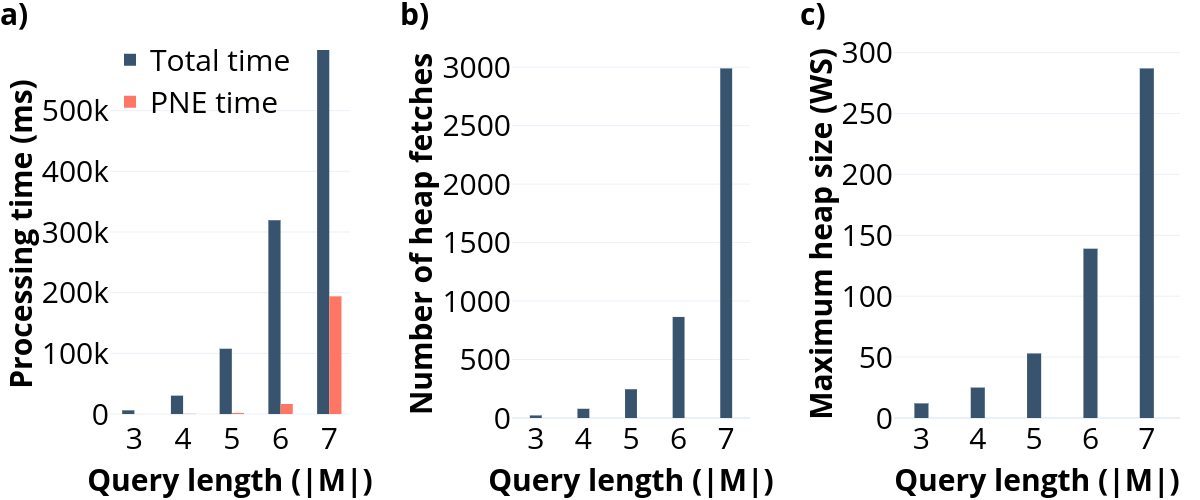
\includegraphics[scale=0.33]{images/eo_length_30.png}
	\centering
	\caption{Equality "operator" - experiments on the query length}
	\label{fig:eo_length}
\end{figure}

In the next set of experiments, shown in Figure \ref{fig:eo_frequency} a), b), c), the "equality" operator was evaluated in terms of the frequency of the categories $c_i$, $c_j$. Frequency relates to the size of each CoI dataset (see Table \ref{dataset}) and is categorized into \textit{low}, \textit{middle} and \textit{high}, for a default query length of 5.  Figure \ref{fig:eo_frequency} b), c) follow the same trend as the experiments for query length. 
As the frequency of the categories, which are selected to be equal, increases, the processing time, the number of heap fetches and the heap's maximum size increase proportionately. This can be explained with the fact that having more points in the CoI dataset of the equal categories increases the search space of the algorithm and respectively more partial routes are being generated, which increases the heap size, number of heap fetches and logically in turn the processing time of the query.

\begin{figure}[h!]
	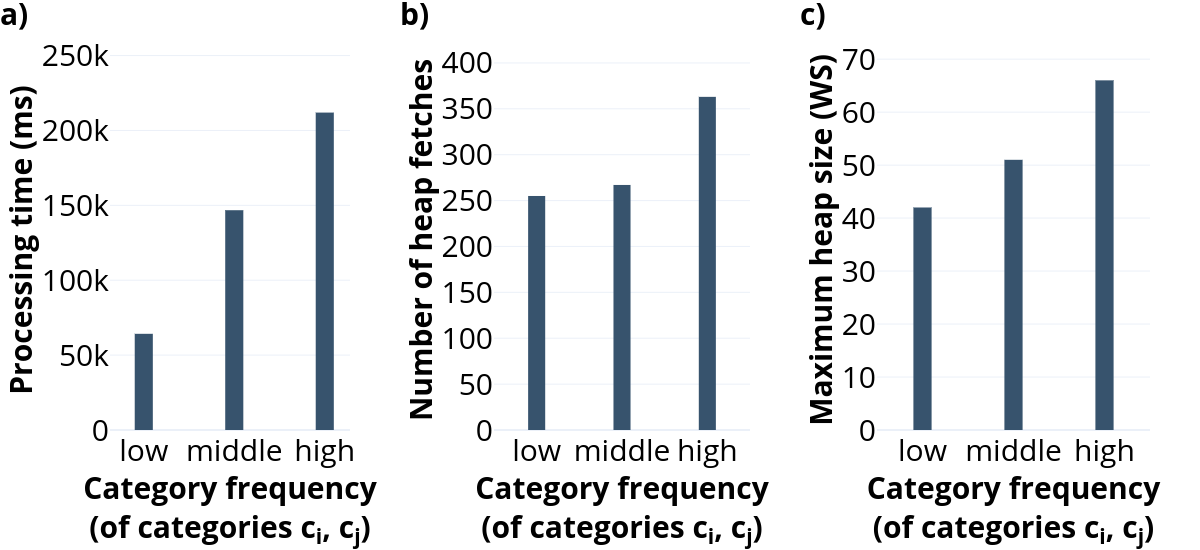
\includegraphics[scale=0.33]{images/eo_frequency_30.png}
	\centering
	\caption{"Equality" operator - experiments on the category frequency of the categories $c_i$ and $c_j$}
	\label{fig:eo_frequency}
\end{figure}

In the third set of experiments, shown in Figure \ref{fig:eo_distance} a), b), c), the "equality" operator was evaluated in terms of the  distance between the categories $c_i$, $c_j$ in the category sequence $M$, which varies from 1 to 3, for a query length of 5. When the distance between them is 0, the result is always found with PNE, therefore we do not consider distance 1 in the experiments. 
As the distance of the categories, which are selected to be equal, increases, the processing time, the number of heap fetches and the heap's maximum size increase proportionately. This stems from the fact that by increasing the distance, the probability that the PoIs at indices $i$ and $j$ would be equal decreases, therefore less of the routes are found in the first step of the algorithm with PNE. This in turn causes the method to continue with the heuristic approach in order to find an optimal route, which increases the processing time, number of heap fetches and also the work space (maximum heap size).

\begin{figure}[h!]
	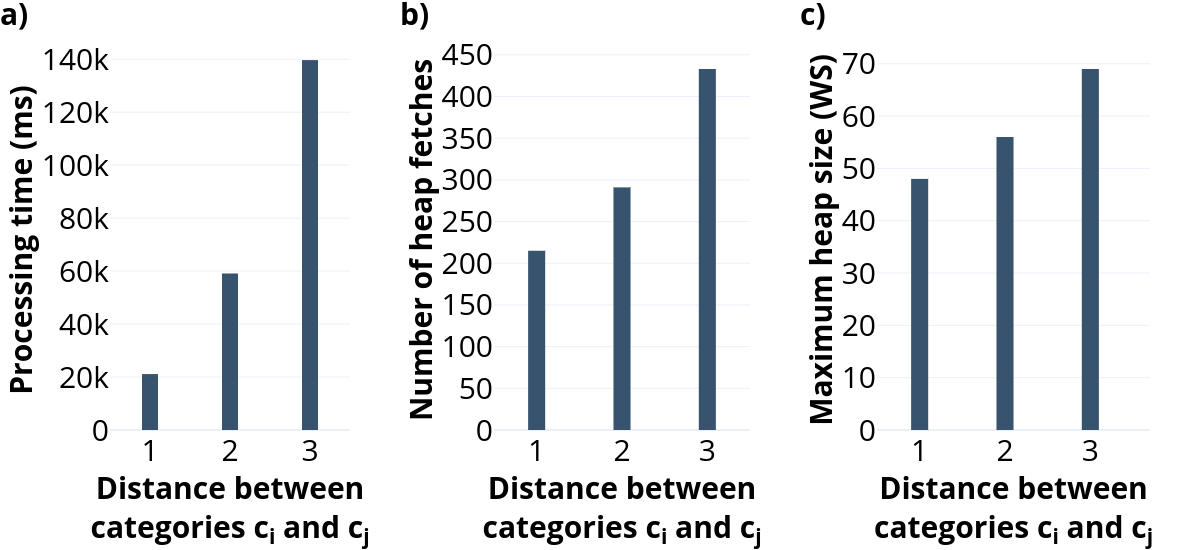
\includegraphics[scale=0.33]{images/eo_distance_30.png}
	\centering
	\caption{"Equality" operator - experiments on the distance between equal categories $c_i$ and $c_j$}
	\label{fig:eo_distance}
\end{figure}

Finally, the last set of experiments, shown in Figure \ref{fig:eo_distance} a), b), c), compares the baseline approach with the proposed approach in terms of the factor query length. It can be seen that the proposed approach outperforms the baseline approach for all values of the query length. Also with increase in the query length, the values for the processing time, the number of heap fetches and the maximum heap size of the baseline approach increase with a more than a linear rate compared to the the proposed approach. For query's length 7 the values for the processing time, the number of heap fetches and the maximum heap size of the baseline approach exceed the graphic's range and are not fully depicted.

In conclusion, the proposed method performs as expected in all studied parameters and outperforms the baseline approach by an exponential amount. 

\begin{figure}[H]
	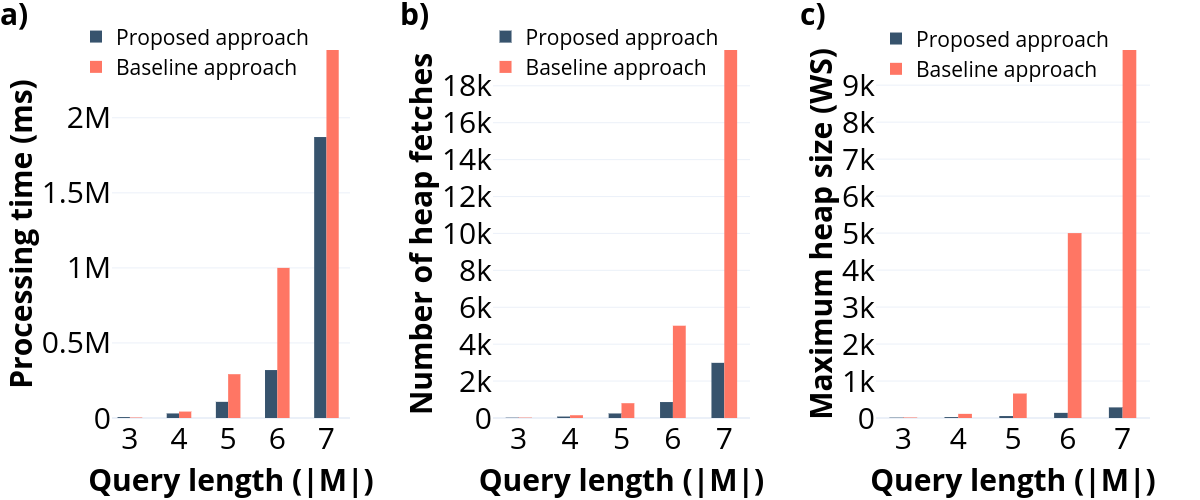
\includegraphics[scale=0.33]{images/eo2_30.png}
	\centering
	\caption{"Equality" operator - comparison experiments on the proposed approach and the baseline approach in terms of query length}
	\label{fig:eo2_length}
\end{figure}


\section{"Inequality" operator}
\label{sec:experimentsNEO}

The "inequality" operator was also evaluated with respect to the effect of following 3 parameters: (1) query length (cardinality of the category sequence $|M|$), (2) the frequency of the categories $c_i$, $c_j$ and (3) the distance between the categories $c_i$, $c_j$ in the category sequence $M$. Categories $c_i$, $c_j$ represent the CoIs for which unequal PoIs should be found.

In the first set of experiments, shown in Figure \ref{fig:neo_length} a), b), c), the "inequality" operator was evaluated in terms of query length, which varies from 3 to 7. As we can see in Figure \ref{fig:neo_length} a), the query processing time increases proportionately to the query length. Similar to the "equality" operator, the response time and the number of heap fetches for a query with length 7 have not been depicted fully in the graphic due to a lack of space, but it can be seen that they increase exponentially with the increase in query length. Figure \ref{fig:neo_length} b), c) follow the same trend of a). As the query length increases, the number of heap fetches and the maximum heap size also increase.

\begin{figure}[H]
	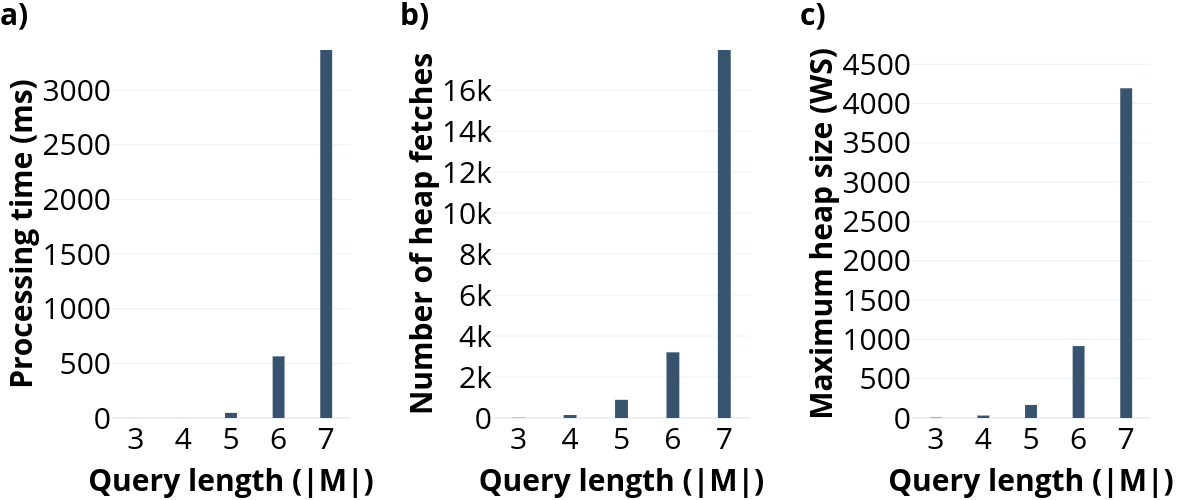
\includegraphics[scale=0.33]{images/neo_length_30.png}
	\centering
	\caption{"Inequality" operator - experiments on the query length}
	\label{fig:neo_length}
\end{figure}

In the second set of experiments, shown in Figure \ref{fig:neo_frequency} a), b), c), the "inequality" operator was evaluated in terms of the frequency of the categories $c_i$, $c_j$, which can be \textit{low}, \textit{middle} and \textit{high}, for a default query length of 5.  
Here we can see more interesting results compared to the "equality" operator. The \textit{low} frequency has higher results on all parameters than the \textit{middle} frequency. This can be explained with the fact that when the categories which have to be not equal are less frequent, then the possibility of PNE reaching a route with different PoIs at places of the not equal categories is lower. In this case the search space of not equal PoIs is larger, compared to when the category of the not equal PoIs has a middle frequency. And when the category frequency is high, if PNE does not directly find a route with equal PoIs then the inequality algorithm must inspect more PoIs. Therefore the algorithm generates more routes and the time increases exponentially. 
The results in \ref{fig:neo_frequency} b), c) are equivalent to the results in \ref{fig:neo_frequency} a). 

\begin{figure}[H]
	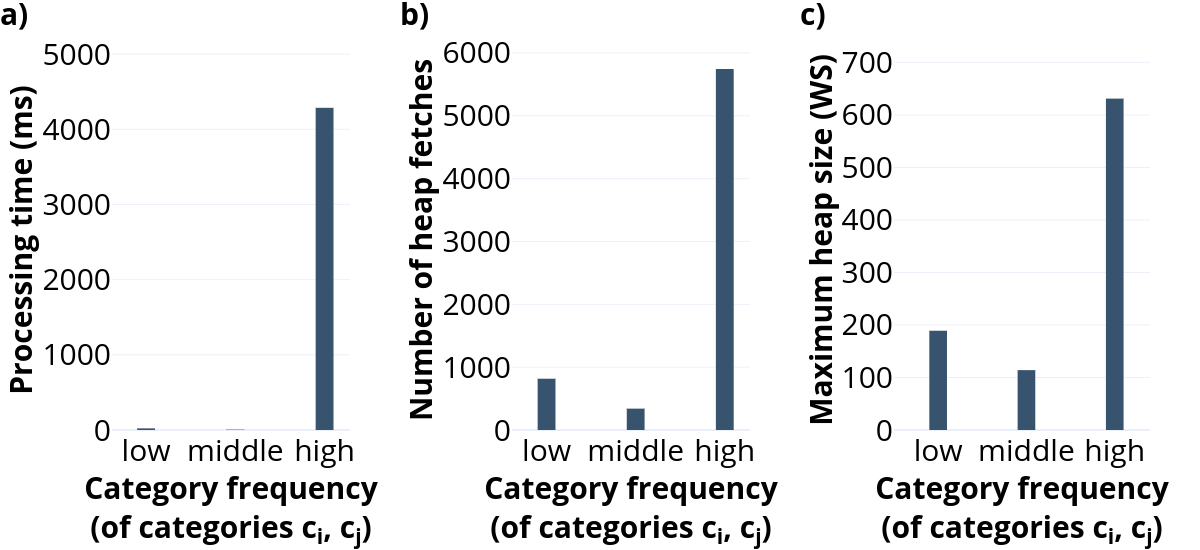
\includegraphics[scale=0.33]{images/neo_frequency_30.png}
	\centering
	\caption{"Inequality" operator - experiments on the category frequency of the categories $c_i$ and $c_j$}
	\label{fig:neo_frequency}
\end{figure}

In the third set of experiments, shown in Figure \ref{fig:neo_distance} a), b), c), the "inequality" operator was evaluated in terms of the  distance between the categories $c_i$, $c_j$ in the category sequence $M$, which varies from 0 to 3, for a default query length of 5.  
Here we can also see more interesting results compared to the "equality" operator. When the distance between the mentioned categories is 0, the result, usually found with PNE, always contains equal points at indices $i$ and $j$. Therefore the algorithm for the "inequality" operator has to inspect more points in order to find the optimal route, in which the PoIs at indices $i$ and $j$ are not equal to each other. This increases the search space and in turn the number of heap fetches, the maximum heap size and the processing time increase as well. For distances 1, 2, 3 no obvious argumentation can be applied, because here we are not able to judge the possibility for equal PoIs objectively.
% Is this argumentation okay?
Nevertheless, all three performance parameters - processing time, number of heap fetches and maximum heap size, follow the same trend and increase proportionately to each other.

In conclusion, our proposed approach performs as expected and for a medium query length (with default length 5) delivers fast results in a response time of a couple milliseconds.

\begin{figure}[H]
	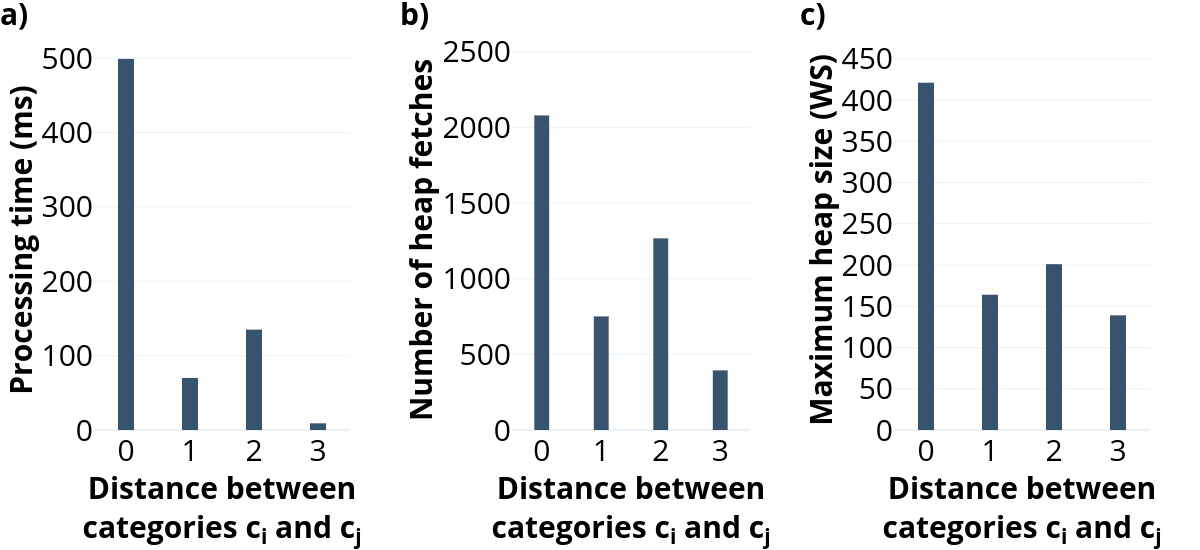
\includegraphics[scale=0.33]{images/neo_distance_30.png}
	\centering
	\caption{"Inequality" operator - experiments on the distance between equal categories $c_i$ and $c_j$}
	\label{fig:neo_distance}
\end{figure}


\section{"Or" operator}
\label{sec:experimentsOr}

The "or" operator was studied with respect to the type and number of operands, for a default query length of 5. Three different types of queries were issued, in which we changed the type and number of or operands in the first OR sequence $OR_1$ of the query, while the other four OR sequences only contained one category sequence with a single category. For \textit{2 simple operands} the first OR sequence contained two category sequences with one single category each, for \textit{3 simple operands} the first OR sequence contained three category sequences with one single category each and for \textit{2 complex operands} the first OR sequence contained two complex category sequences with two categories in each. In this way the complexity of the problem was gradually increased to see how the baseline approach compares to proposed approach of the algorithm.  
Figure \ref{fig:or} a), b), c) shows that the processing time, number of heap fetches and maximum heap size increase proportionately with the complexity of the query. As seen from the experiments the proposed approach is also by magnitudes faster with more than a linear rate and also more efficient in terms of heap size, as the complexity of the query increases. 

\begin{figure}[H]
	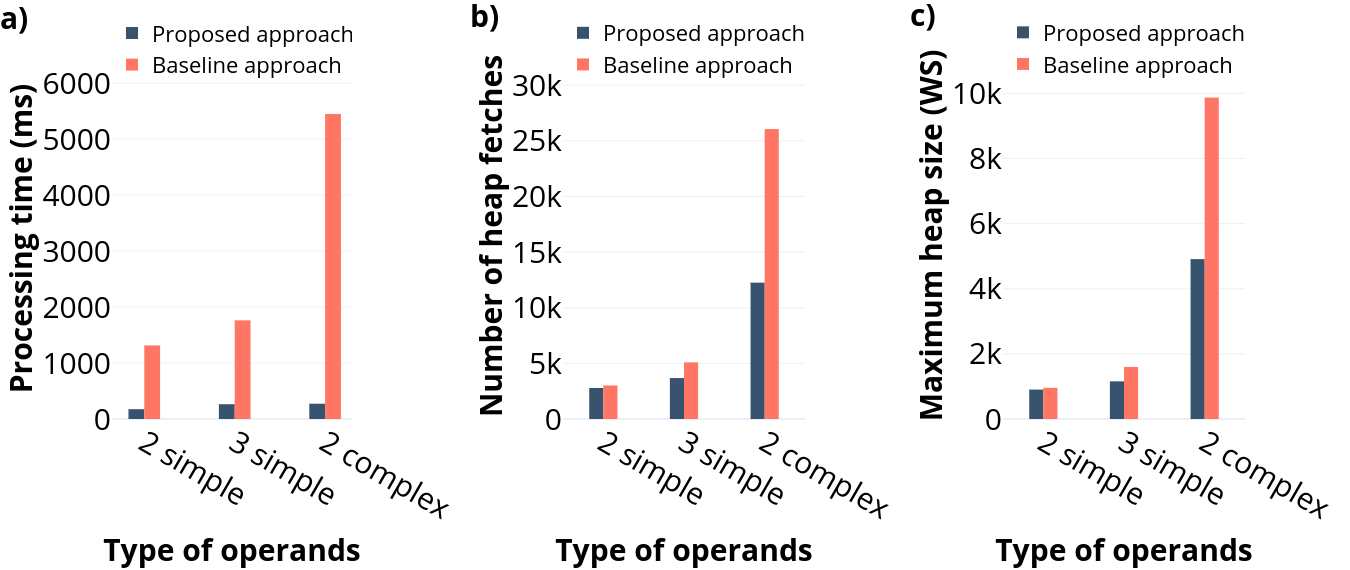
\includegraphics[scale=0.29]{images/or_30.png}
	\centering
	\caption{"Or" operator - experiments on the type and number of operands}
	\label{fig:or}
\end{figure}


\section{"Order" operator}
\label{sec:experimentsOrder}

The "order" operator was evaluated with respect to the number of fixed positions in a default query length of 5. The number ranges between 0 and 3. When the number of fixed positions is 4 or 5, the problem can be solved with simple PNE, therefore we do not consider these numbers in the experiments. The complexity of the problem is gradually decreased to see how the baseline approach compares to proposed approach of the algorithm.  
Figure \ref{fig:order} a), b), c) shows that the processing time, number of heap fetches and maximum heap size decrease proportionately with the complexity of the query. For unordered queries with 0 fixed positions the values for the processing time, the number of heap fetches and the maximum heap size of the baseline approach exceed the graphic's range and are not fully depicted. But as can be seen from the experiments the proposed approach is with an exponential rate faster and also more efficient in terms of heap size. \newline

\enlargethispage*{30pt}

\begin{figure}[H]
	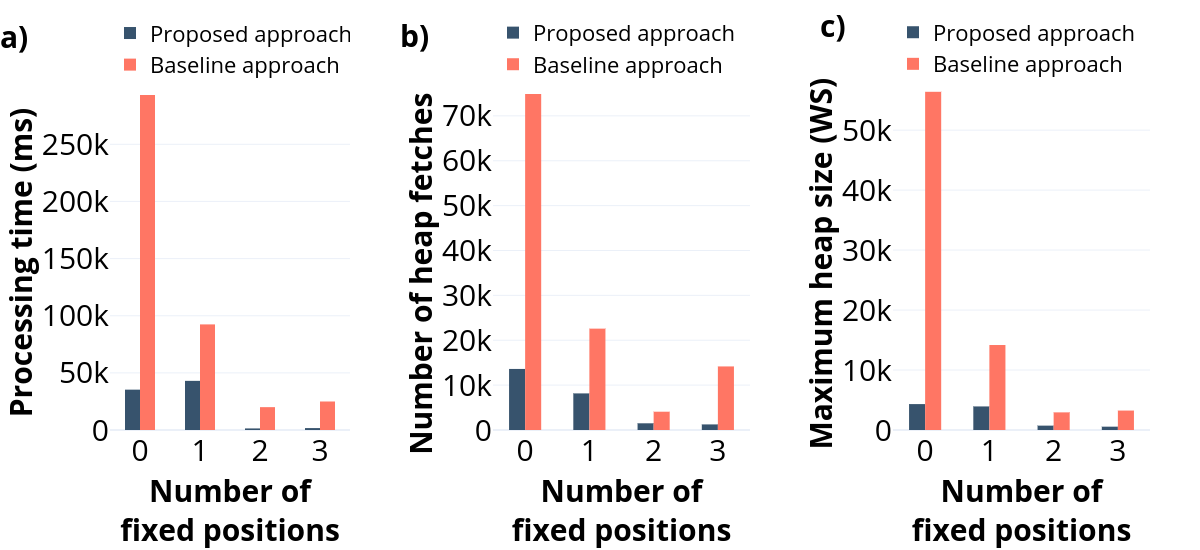
\includegraphics[scale=0.33]{images/order_30.png}
	\centering
	\caption{"Order" operator - experiments on the number of fixed positions}
	\label{fig:order}
\end{figure}

\section{Evaluation}
\label{sec:eval}

We can conclude that we have successfully developed four operators for the route query language, which perform as expected in all our quantitative criteria such as time, heap fetch operations and required work space. They also outperform the baseline methods with more than a linear rate with increasing of the search space and therefore prove to be effective solutions.

It is important to mention that the implemented approaches could easily be modified to return \textit{k} number of optimal routes, if the user may be interested in this. Also, the proposed approaches are not only limited to using the route length  as measure criteria. Alternative to this could be the route duration. In different scenarios, the methods could also be extended to consider PoI ratings and subjective preferences such as preferred length of the route or traveling time to  specific location could be considered as well.  

% We do not report I/O cost separately, because for all methods in all settings, the I/O time is no more than a few milliseconds; i.e., at least an order of magnitude lower than the total response time. 
% Summing up, unresolved problems and further research
\chapter{Conclusion and Future work}
\label{sec:conclusion}
\enlargethispage*{30pt}

We studied the different types of route queries, that are currently present in the research, and we identified the lack of a query language designed for the user's specific needs for flexibility when it comes to route queries. In order to attempt to fill this gap, we proposed four operators, which are specifically designed for route queries in metric spaces and the prime factor upon which routes are quantified is travel distance. 
We first presented the equality operator, which was designed based on the PNE approach \cite{OSR} and a heuristic to reduce the search space. We showed through evaluation experiments that the proposed approach outperforms the baseline approach in all of the experiment parameters. Next, we introduced the not-equality operator as extension to the equality operator. For this operator we modified the PNE algorithm in order to get the desired result. Furthermore, we presented the or operator, which strives to give the user maximum flexibility when it comes to building a multiple-option route query. For this operator we developed an algorithm to work with multiple query options simultaneously and when we compared it with the baseline approach, it proved to perform significantly better, especially when many or operands are presents. Last but not least, we designed the order operator, which gives the user the ability to construct partially or even fully not sequenced route query. This approach was also designed similarly to the or operator by developing a method to handle and compare multiple query options at once. When comparing with the baseline approach, we concluded that the proposed approach performs exponentially better than the trivial solution whenever the number of ordered elements decreases.

With these finding in mind, we consider our work to has successfully delivered four query language operators that could be implemented and used in location based services. In comparison with other attempts at solving the multi-rule route queries \cite{multi}, our proposed approaches deliver an optimal result. It is important to note, however, that the mentioned operators are definitely not a complete set of query language operators, but they represent the four ones, that have proved to be the most desired in query language overall and therefore fulfill the user requirements the most. Nevertheless, while researching the topic of route queries, we came up with multiple ideas for operators that could be further researched and implemented. Such operator is for example the hops operator, with which the user can explicitly define how many location visits he wants to make between two categories in the category sequence. This operator is very similar to the order operator and could be designed similarly. Furthermore, an operator could be developed, with the help of which the user can specify necessary categories, which must be present in the final result. Considering this, the query route would only contain the PoIs of unnecessary CoIs, if these are situated on the way between the necessary points and the route's length does not increase with by adding them. Although still useful as a separate operator, the user could also achieve the same with our already developed or operator. \newline
Another ideas for operators, which are targeted more towards the semantic hierarchy of the categories in the user-specified category sequence, could be the and and not operators. These two operators could be applied to specific categories in the user query's category sequence and could be useful in the case that a single PoI has many category types. For example of the and operator, a user may want to go to a cafe, that is also a restaurant, or in the case of the not operator, he may want to visit a restaurant, which is also specifically not categorized as a coffee shop. \newline
All of these mentioned operators could be also inspired by the PNE approach that we used for the four operator in this thesis. But another solution could be to expand on the \textit{Skyline Sequenced Route Query} (SkySR) \cite{skyline}. This method searches for routes based on the Skyline concept, which entails finding routes that are not worse than any other routes in terms of theirs scores - route length and semantic similarity. This could be another alternative to give more flexibility to the user by making use of the semantic similarity of CoIs. An operator that could be useful in this case is the perfection operator, applied to categories in the category sequence. With this operator, a user can specifically force the Skyline algorithm to match the category to which the operator has been applied perfectly in terms of semantic similarity. Finally, there is probably many other operators that would come up with further scientific work and research on the topic of route queries and the ones we summarize here are only our suggestions to the topic. For future work, it would be also interesting to extend the proposed algorithms to also support dynamic road networks, in which traffic information is provided (e.g., travel time, traffic congestion, etc.).

In conclusion, we think that with the development of four operators for the route query language we have successfully contributed to this field of research. We have also managed to identify linked topics for further study and to make recommendations on how to expand the query language. 

\pagebreak


\listoffigures
\listoftables
\listofalgorithms

\backmatter    
%\chapter{Bibliography}
\phantomsection
\addcontentsline{toc}{chapter}{Bibliography}
\bibliography{diploma_thesis}
\end{document}
